\newpage
\chapter{Design Changes}
\label{chap:design_changes}
% what major design changes have been introduced since the CDR report? Argument why these changes were necessary. Also, will be good to include test results (functionality, weight, performance etc.) which are not documented in the CDR report.
%
%
\section{Project Schedule, Resources and Goals}
\label{sec:project_changes}
%responsible: Morten
%
As previously stated in \cite{CDR}, the U-SPACE project was initially substantially delayed due to bureaucratic challenges in course registrations and subsequent release of project budget. This resulted in a reformulation of the system concept going from a custom designed helium envelope to a \ac{COTS} blimp provided by Esrange Space Center.

In June 2012, many of the U-SPACE team members left Kiruna to pursue summer internships and prepare for their 3rd semester outside Sweden. Work on the project over the summer holiday was restricted since \ac{LTU} personnel was unavailable thus making ordering of new components impossible. Work on U-SPACE began again in September 2012, when Jan and Pedro returned to Sweden and Omair officially joined the project. At this point, Morten took over the full project management responsibilities and also remained responsible for the power subsystem, Jan became the lead responsible for the attitude sensors and payload, Omair responsible for all on-board telemetry handling, telecommunication and ground station and Pedro responsible for the mechanical structure, thermal design and motors.

During autumn in Kiruna, the sun sits very low on the horizon and is almost completely absent during winter. It was therefore decided, for the first prototype, not to implement the solar array and related electronics. Instead, the goal would be to realize an indoor battery powered flight. This also reduced the work load as was required due to the fewer people now working on the project.

Weekly status meetings were held with project supervisors, but internal meetings were only held on a need-basis since the group just counted four people and were often already sitting together in the Viking project room. 
Due to some misunderstandings of the initial budget, it was approved by the supervisors to increase the project budget for the four remaining students from 2000 SEK to 2500 SEK per student. 


\section{Electrical Power Subsystem}
%responsible: Morten
%
Due to the issues discussed in section \ref{sec:project_changes}, the full amount of solar cells was not ordered. However, it is still believed that the cells tested and discussed in \cite{CDR} are suitable for this project.

One great challenge in the U-SPACE design is to keep the system mass low. Therefore, all custom electronic boards are built on extra thin \ac{PCB}(0.4 mm), using mainly \acp{SMD}, connectors and mechanical mountings made in plastic materials.

In the final circuit layouts, it was decided to place the \ac{BCR} and \ac{SAR} on separate \acp{PCB}. Additionally, a small temperature sensor board was built. The following sections describe the features and circuit diagrams of each of these boards.
%
%
%
\subsection{Battery Charge Regulator}
\label{sec:changes_BCR}
%
The \ac{BCR} is responsible for handling safe charging of the \ac{LiPo} battery and power distribution to the motors and to the logic power supplies. Table \ref{tab:BCR_features} lists the main features of the final \ac{BCR}.
%
\begin{table}[H]
\centering
\caption{\ac{BCR} features}
\label{tab:BCR_features}
\begin{tabular}{p{0.42\textwidth}p{0.18\textwidth}p{0.35\textwidth}}
\hline
\textbf{Feature/Specification} & \textbf{Value} & \textbf{Comments}\\
\hline
Max output current & 20 A & All outputs combined \\
Output voltage & 6-8 V & Unregulated \\
Input voltage & 9.2-9.5 V & Higher voltage may lead to overheating\\
%Weight & ??? & \\
Under voltage protection & $V_{BATT}$ < 6.0 V & Only cuts off motor outputs \\
Short-circuit protection & $I_{SC}$ > 15 A & Only on motor outputs \\
Thermal monitor and charge cut-off & & \\
Automatic charge control &  & Constant current, constant voltage and trickle charge\\
Charge inhibit by telecommand & & \\
Power cut-off by telecommand & & Only motor power outputs\\
Charge status telemetry & &\\
Charge/discharge current monitoring & & \\
Battery cells voltage monitoring & & \\
\hline
\end{tabular}
\end{table} 
%
\noindent
The main changes to the \ac{BCR} include added telemetries, telecommands and protection circuits. The short-circuit and under-voltage protections only work on the motor power outputs. This is based on the philosophy of preventing an error in the motor supply propagating to the supply of the onboard computer which would result in complete loss of communication, control and monitoring of the system. The logic power supplies have their own short-circuit protection (fuses) and a battery undervoltage situation can be detected onboard and the computer could be programmed to enter a low power consumption mode (sleep mode etc.). At a battery voltage lower than about 5.7 V, the linear 5 V regulator will inherently cut off logic supply.\\\\
%
All \ac{BCR} functionalities have been tested and verified at room temperature conditions.
%
%
%
\begin{figure}[H]
\begin{minipage}[t]{\linewidth}
\centering
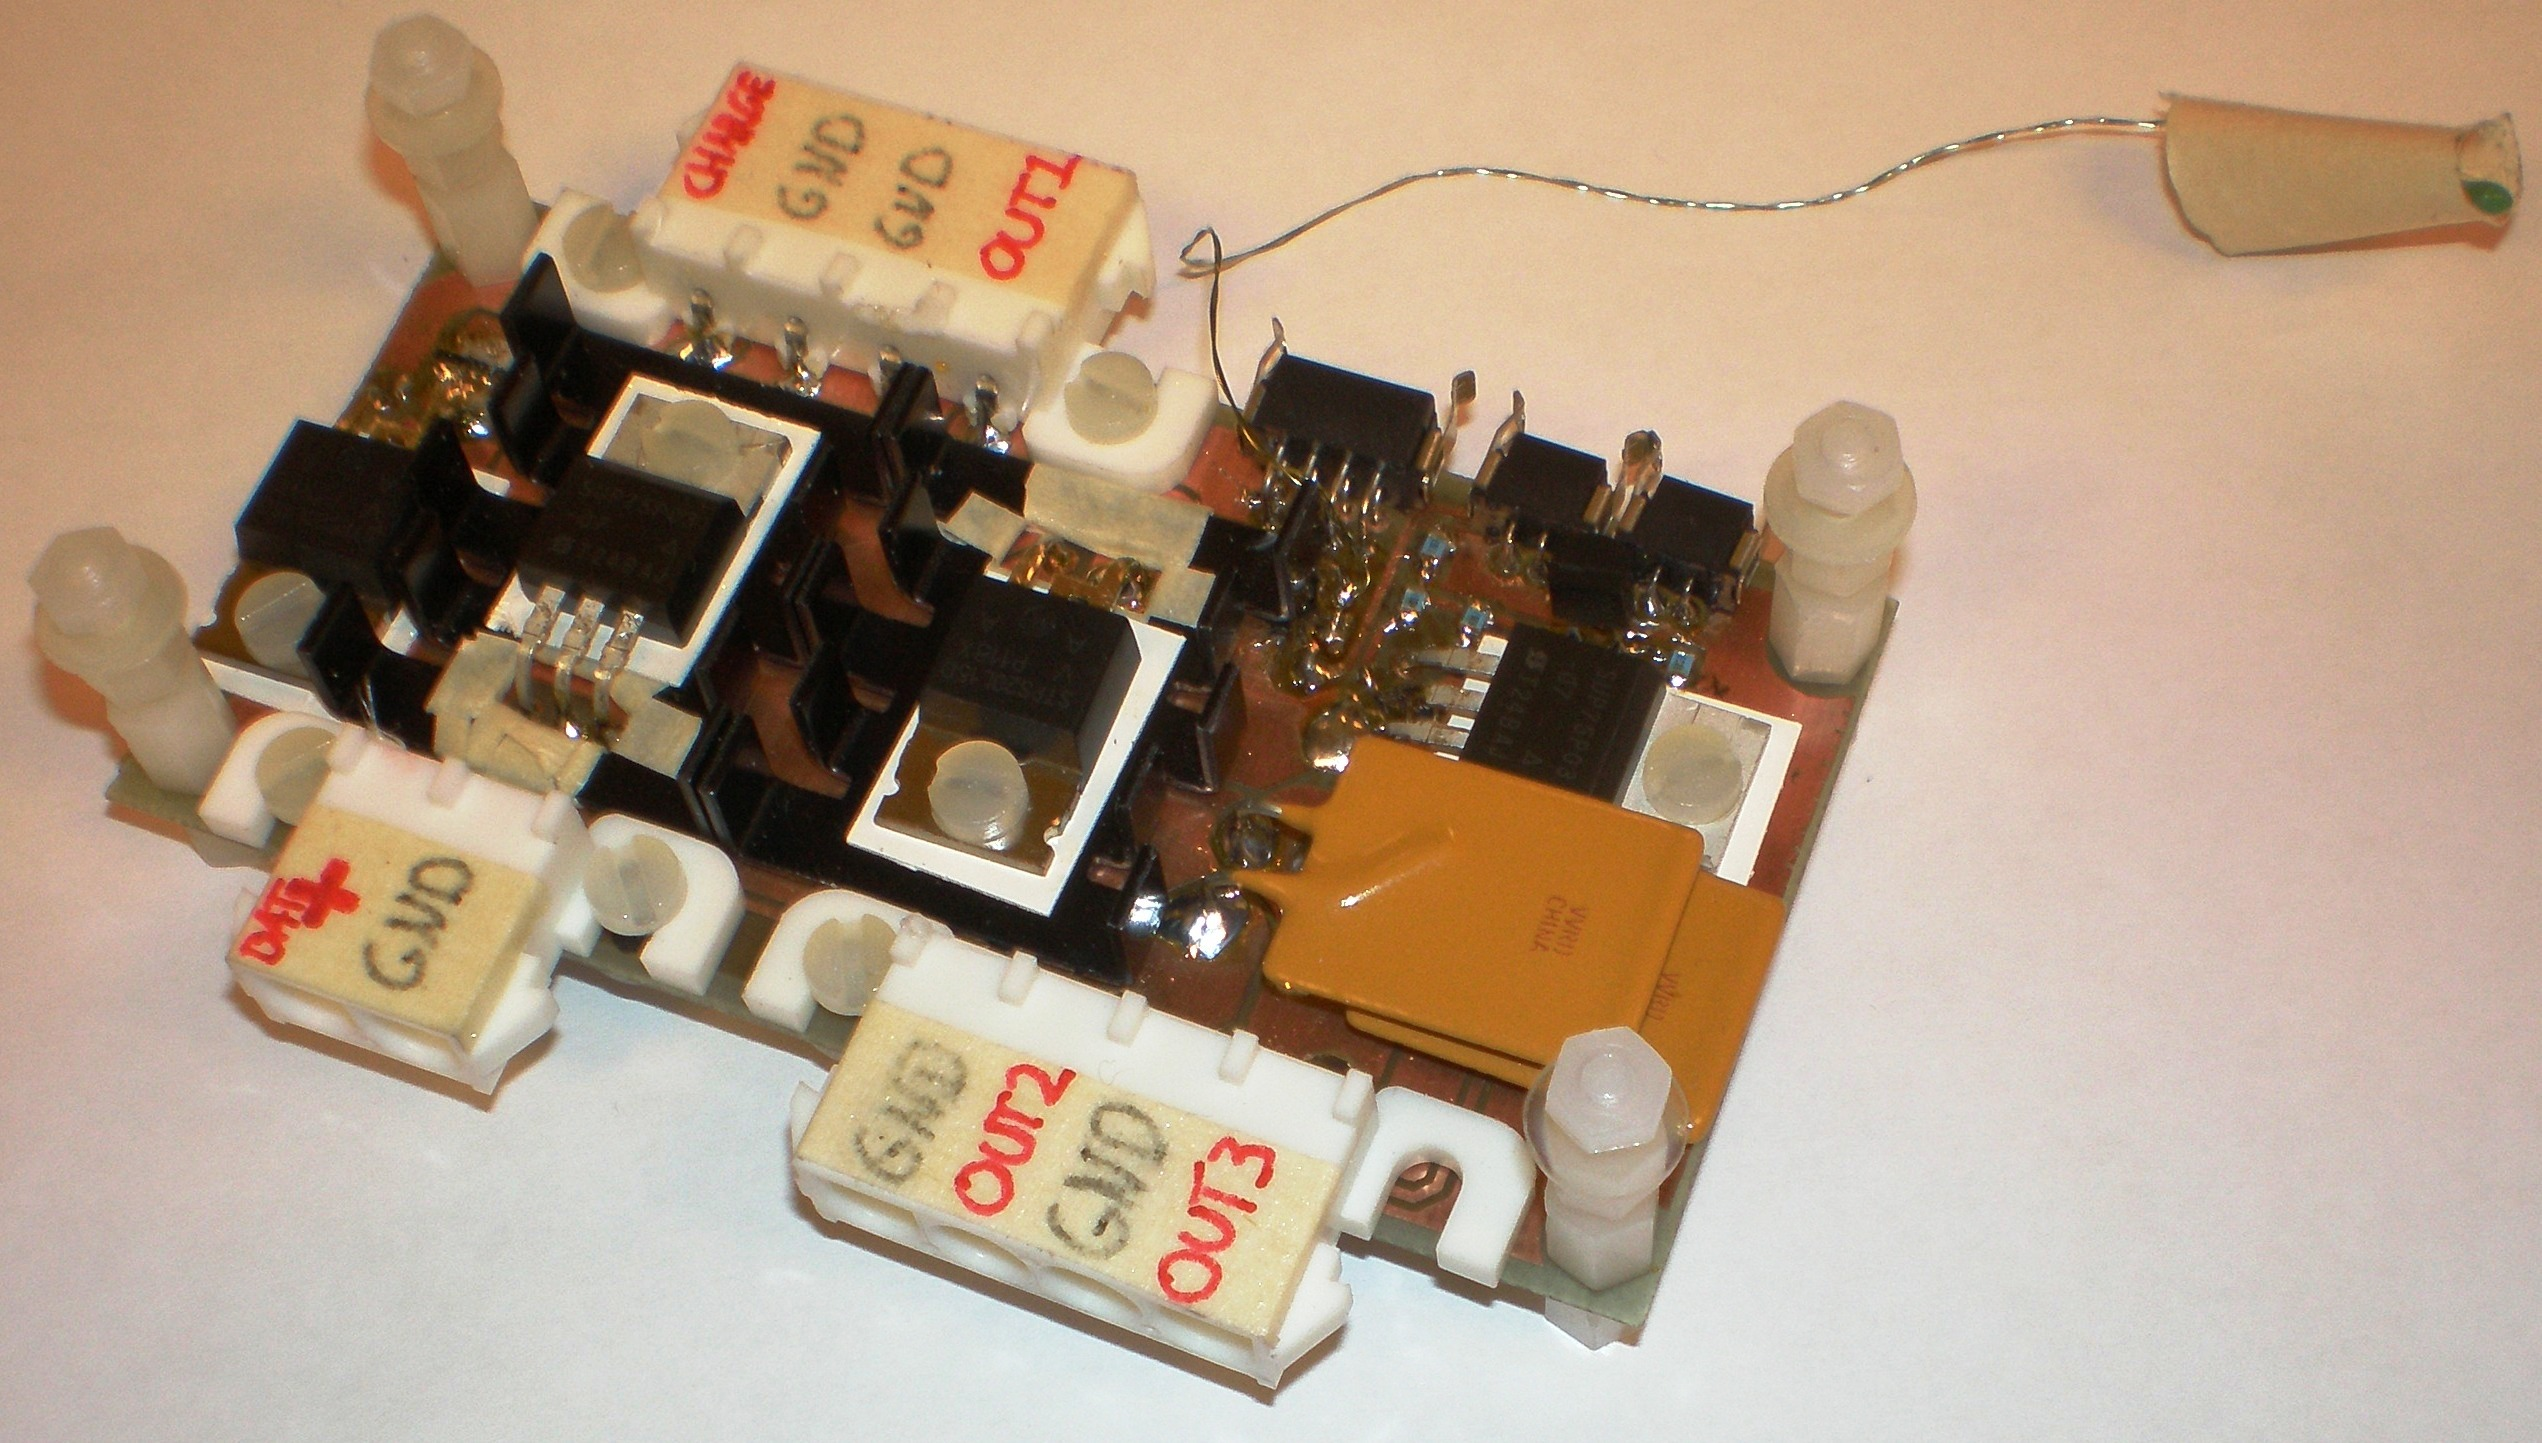
\includegraphics[width=0.7\textwidth]{figures/fig_BCR_top}
\end{minipage}
\\[1mm]
\begin{minipage}[t]{\linewidth}
\centering
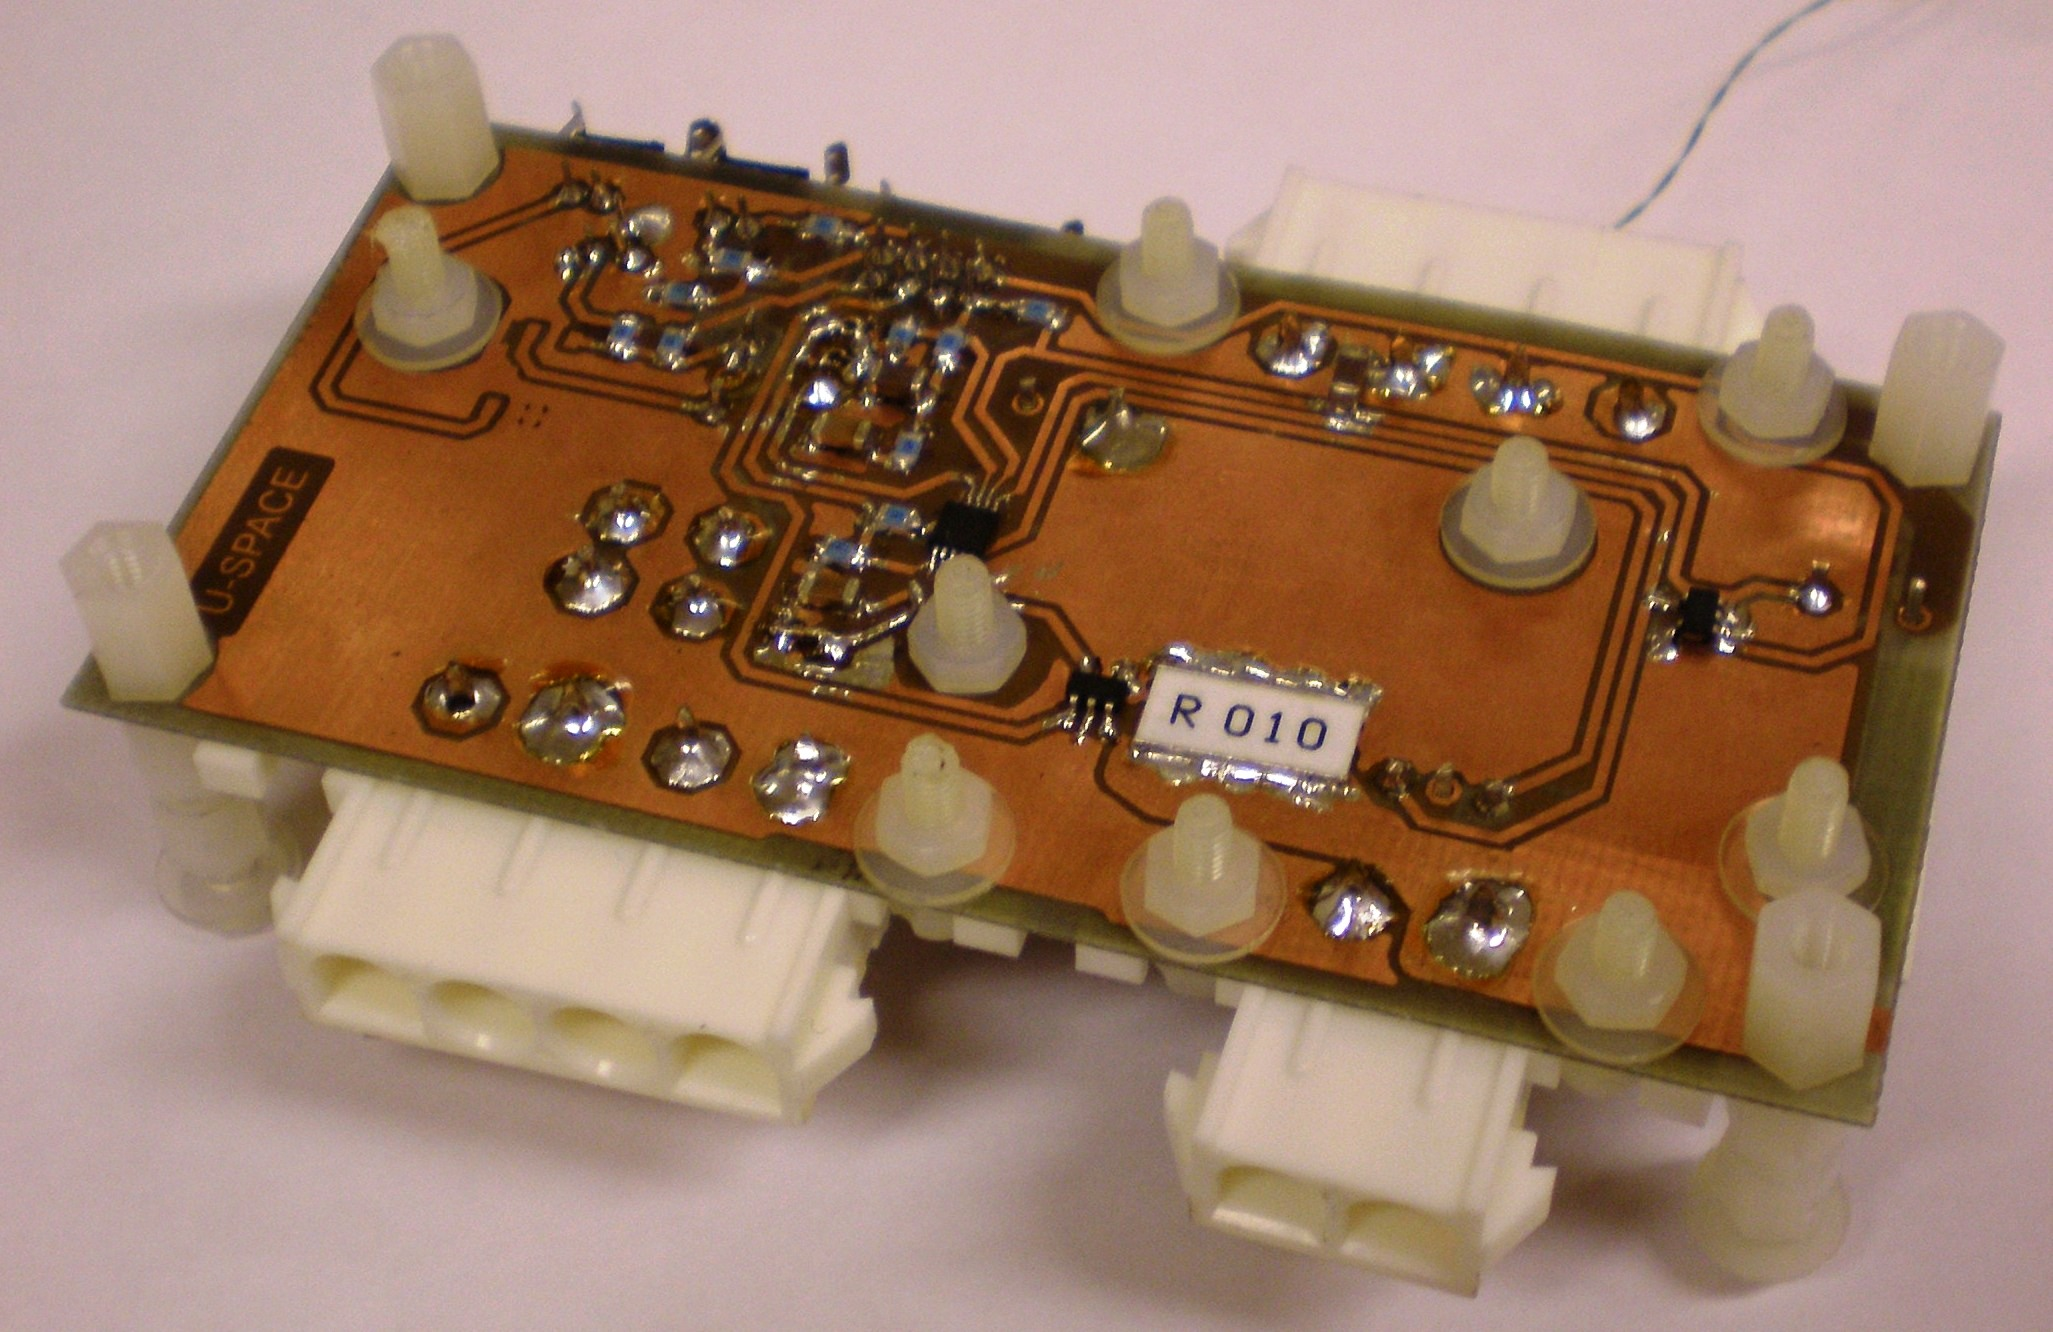
\includegraphics[width=0.7\textwidth]{figures/fig_BCR_bottom}
\end{minipage}
\caption{\acl{BCR} final board}
\label{fig:BCR_top_bottom}
\end{figure}
%
\begin{figure}[H]
\centering
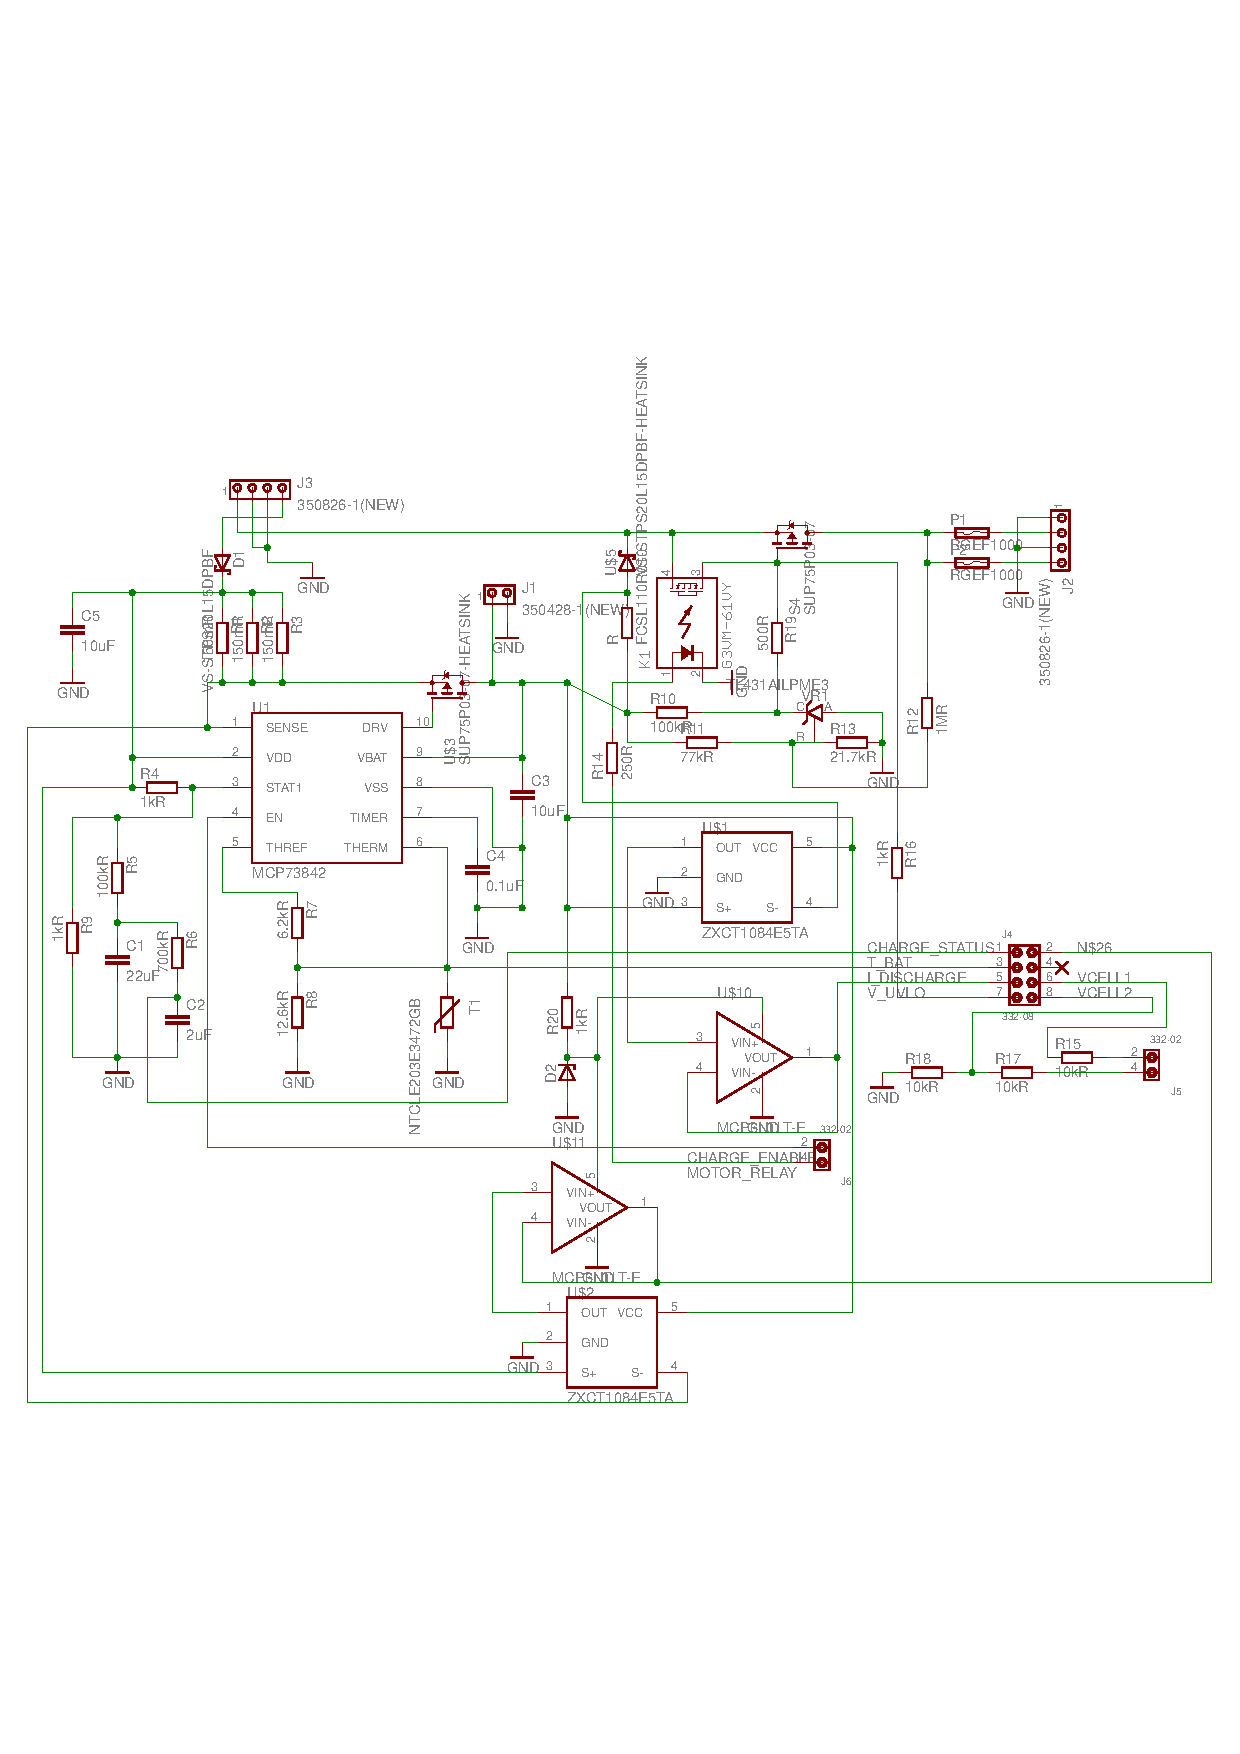
\includegraphics[width=\textwidth]{figures/fig_Schematic_BCR}
\caption{Schematic of the \acl{BCR}}
\label{fig:BCR_Schematic}
\end{figure}
%
%
\subsection{Solar Array Regulator}
%
%
As discussed in section \ref{sec:project_changes}, it was decided not to implement the \ac{MPPT} and DC-DC buck converter for the solar array. The circuit layout of the \ac{SAR} board in  figure \ref{fig:SAR_top_bottom} shows empty space on the \ac{PCB} for later adding on these circuits. Components for implementing the DC-DC converter are already available, but the \ac{MPPT} components must first be ordered.
%
%
In this prototype version, the \ac{SAR} thus only works as a logic power supply to the onboard computer and electronics.
%
%
\begin{table}[H]
\centering
\caption{\acl{SAR} features}
\label{tab:BCR_features}
\begin{tabular}{p{0.42\textwidth}p{0.18\textwidth}p{0.35\textwidth}}
\hline
\textbf{Feature/Specification} & \textbf{Value} & \textbf{Comments}\\
\hline
Output voltages & 3.3 V and 5.0 V & Regulated \\
Maximum output currents & 1.0 A and 1.2 A & Limited by linear regulator and fuse respectively \\
%Weight & ??? & \\
Output currents monitoring & & \\
Output voltage monitoring & & \\
Short circuit protection & $I_{SC}$ > 1.2 A & Both outputs \\
Quiescent current (standby) & 14 mA & \\
\hline
\end{tabular}
\end{table} 
%
%
\begin{figure}[H]
\begin{minipage}[t]{\linewidth}
\centering
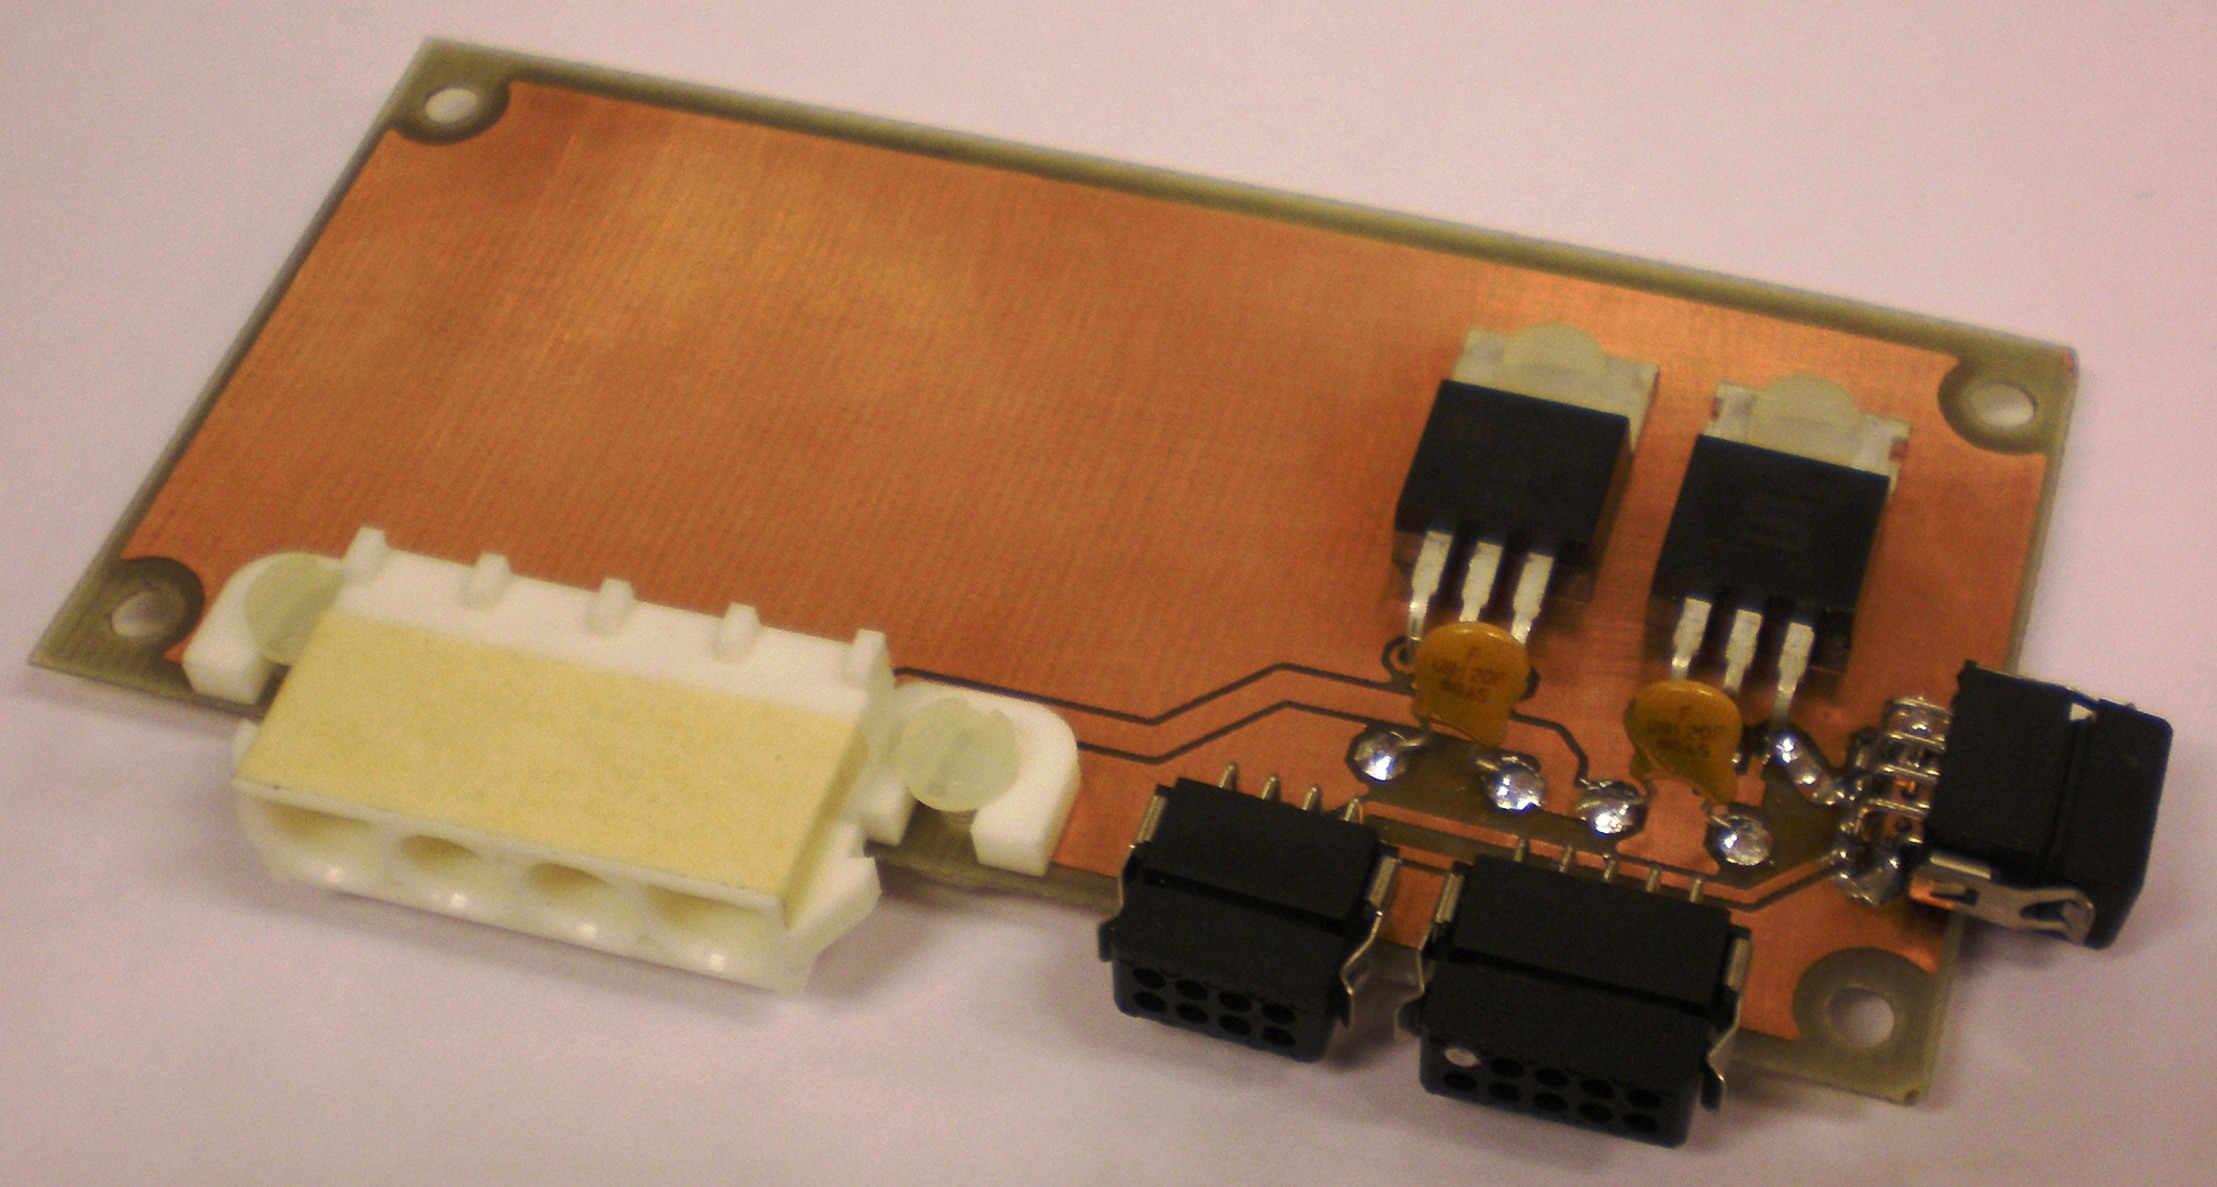
\includegraphics[width=0.7\textwidth]{figures/fig_SAR_top}
\end{minipage}
\\[1mm]
\begin{minipage}[t]{\linewidth}
\centering
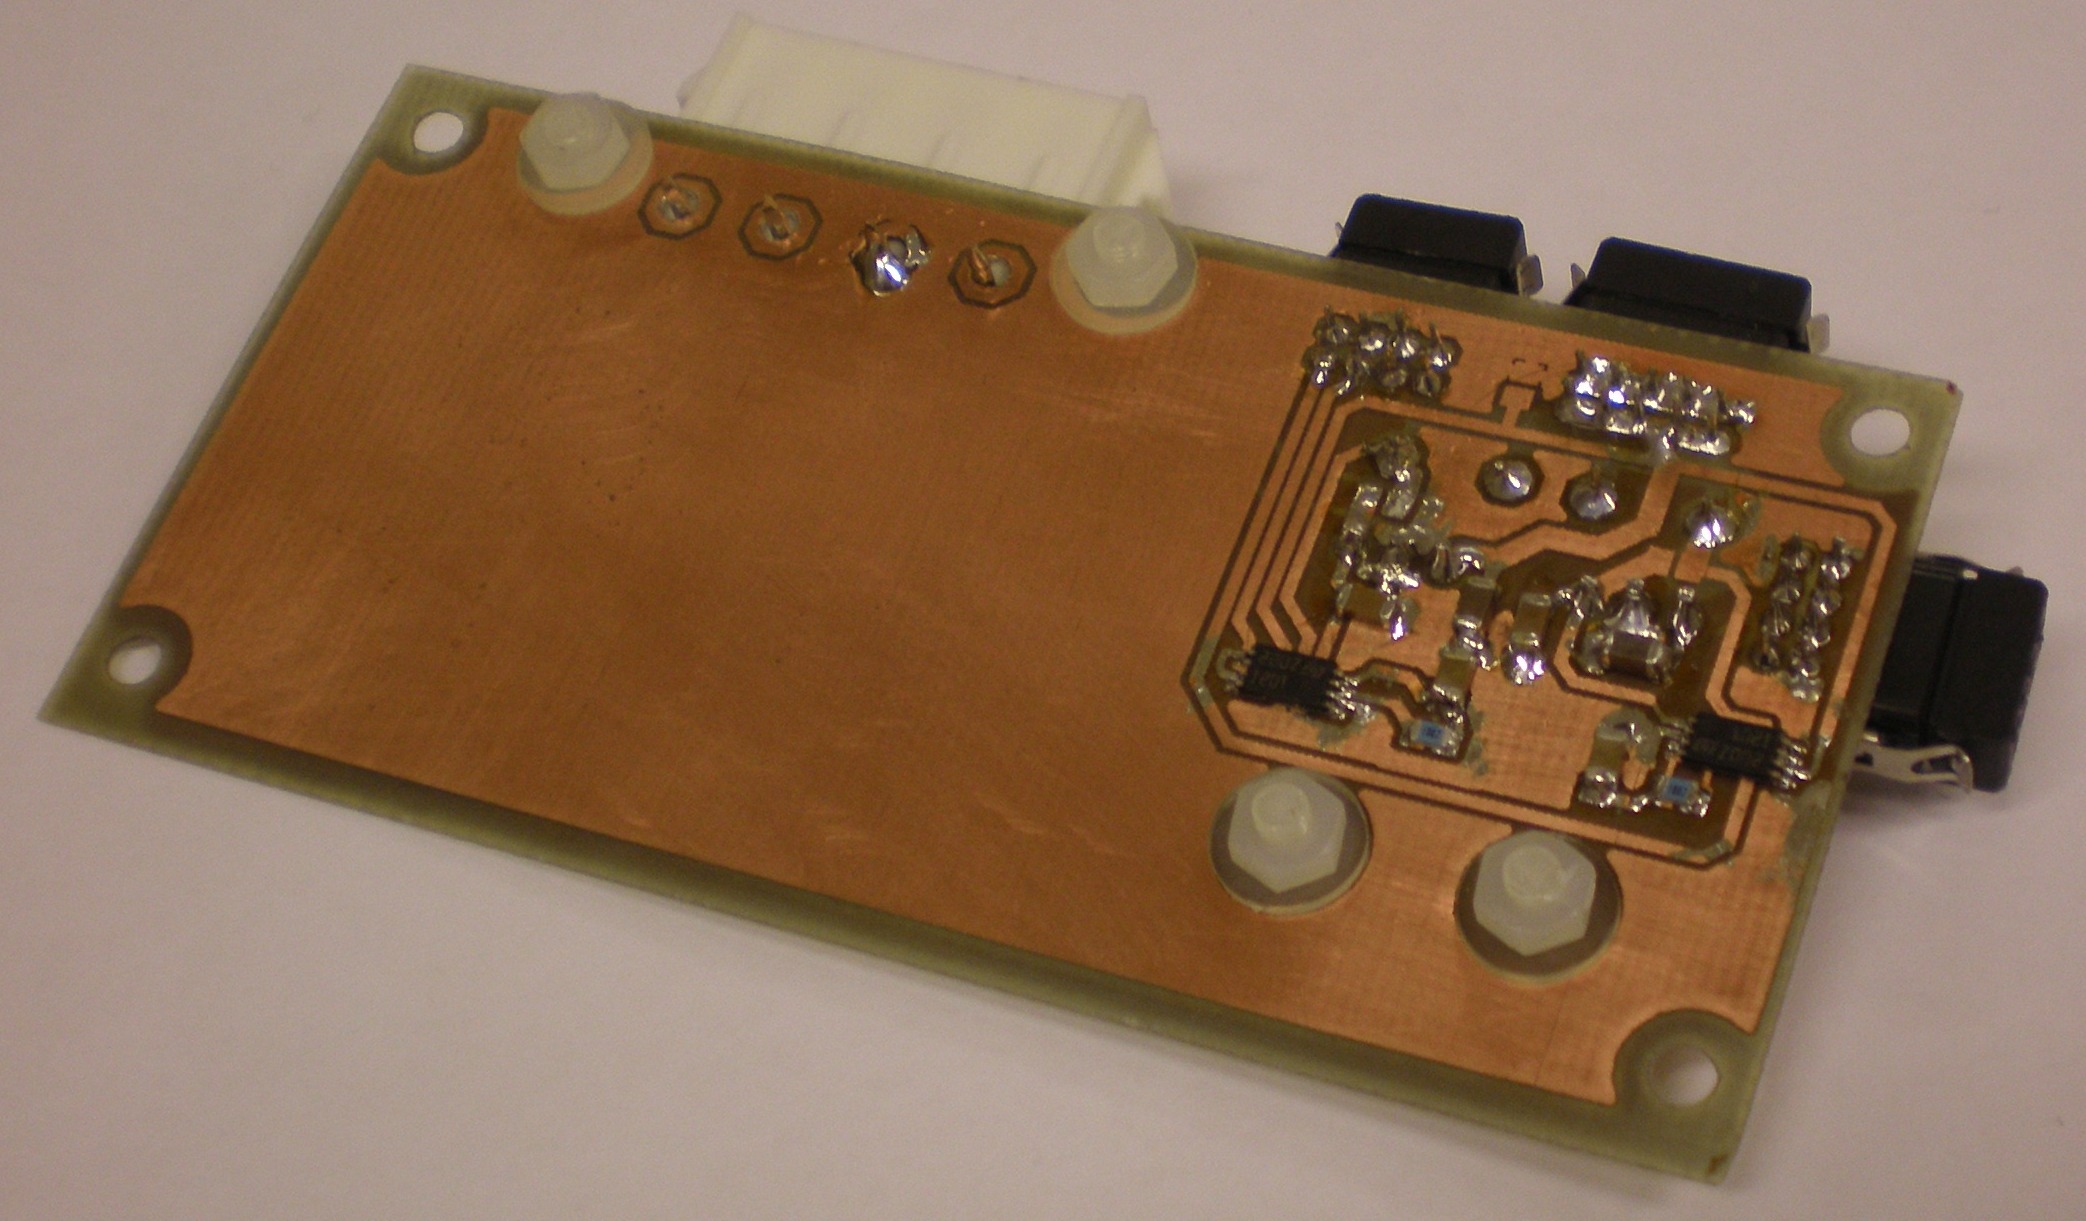
\includegraphics[width=0.7\textwidth]{figures/fig_SAR_bottom}
\end{minipage}
\caption{\acl{SAR} final board}
\label{fig:SAR_top_bottom}
\end{figure}
%
\begin{figure}[H]
\centering
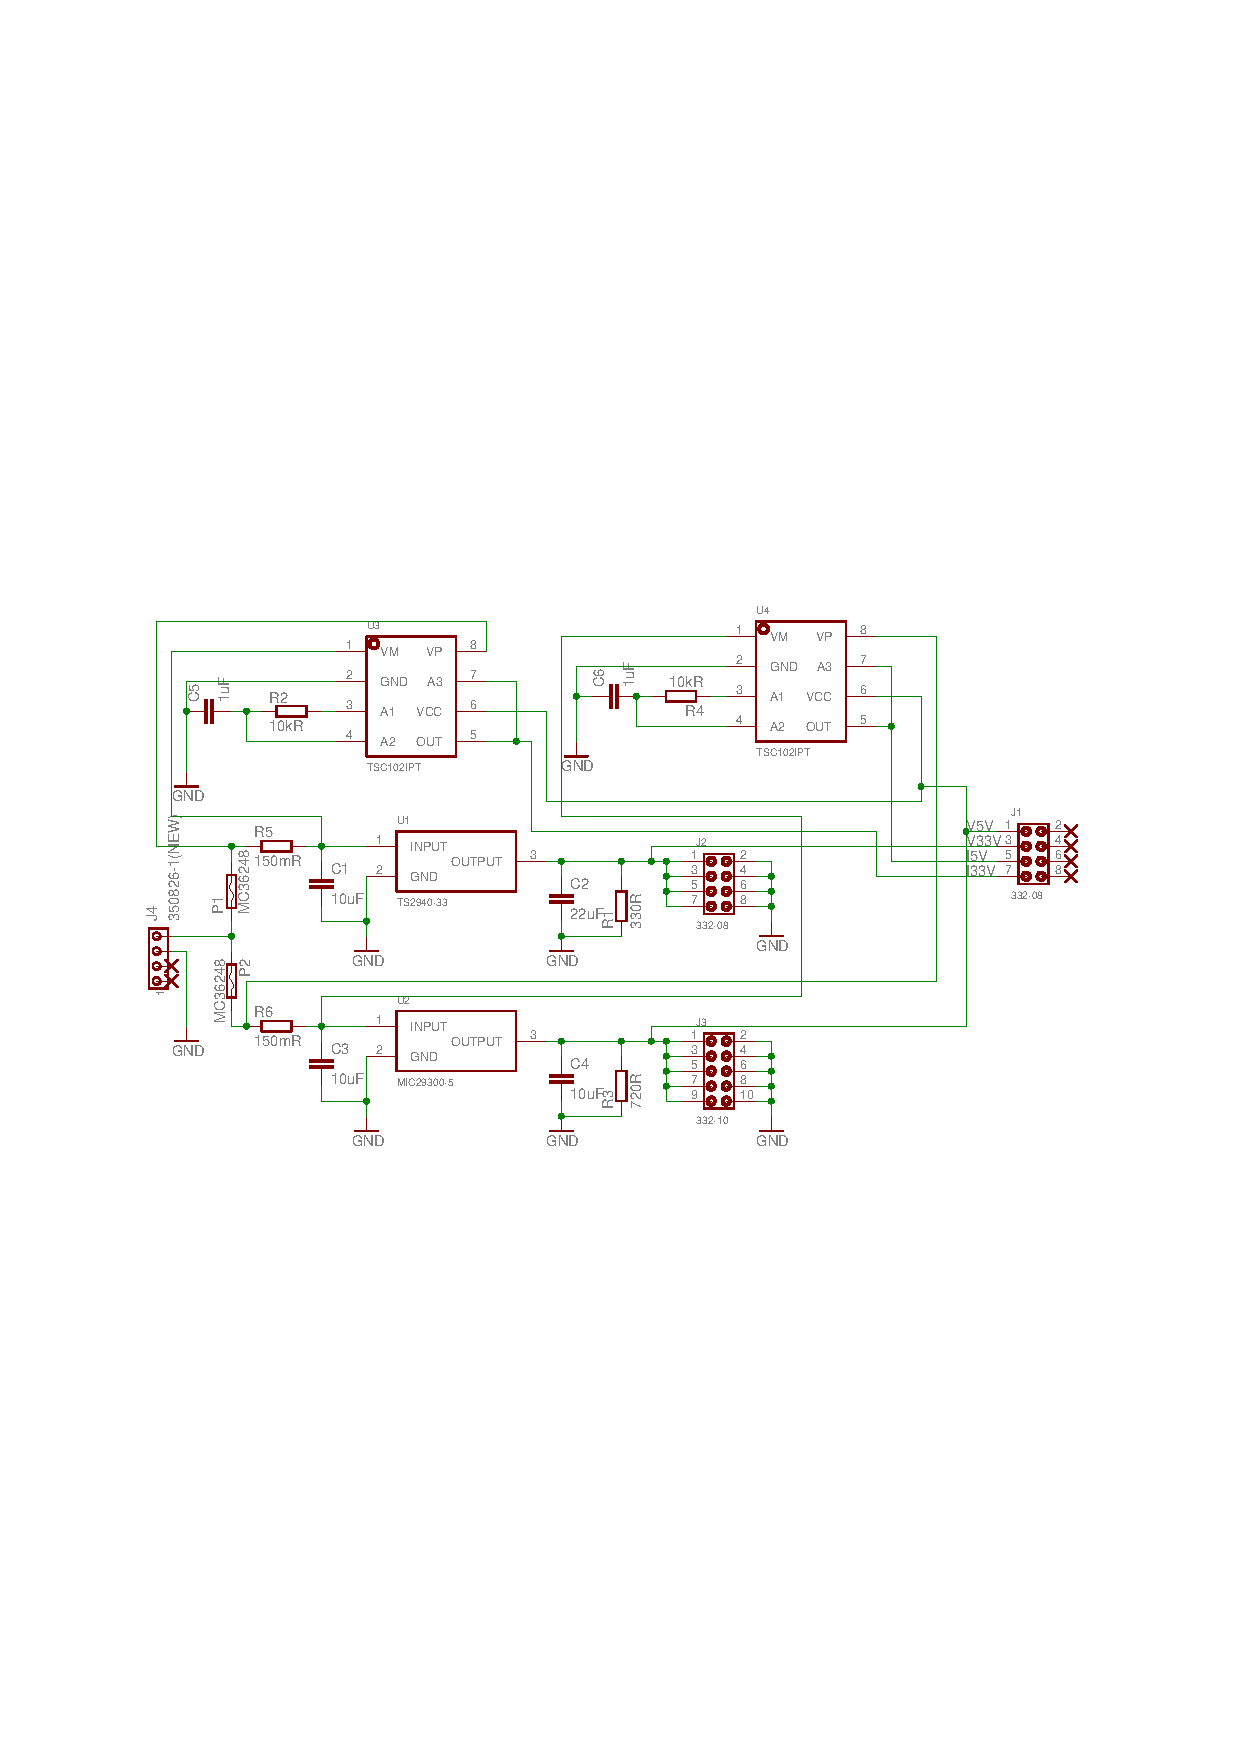
\includegraphics[width=\textwidth]{figures/fig_Schematic_SAR}
\caption{Schematic of the \acl{SAR}}
\label{fig:SAR_Schematic}
\end{figure}
%
%
\subsection{Temperature Sensor Board}
%
When flying U-SPACE outdoors on both warm and cool days, one concern is to maintain the cargo bay temperature within specification of the battery. Even though the first goal was an indoor flight in a heated hangar, a small temperature sensor board was added to monitor the temperatures inside and outside the cargo bay. Up to eight temperatures can be monitored. Temperature monitoring of the motors was also planned, however not implemented. The reason for this was that, due to mass constraints and the long wires needed to reach the motors, very thin wire was required. The wire bought for this purpose proved to be impractical to connect to a connector plug. Hence it is recommended for future designs only to use connectors and wires which are stated as compatible.
%
\begin{figure}[H]
\centering
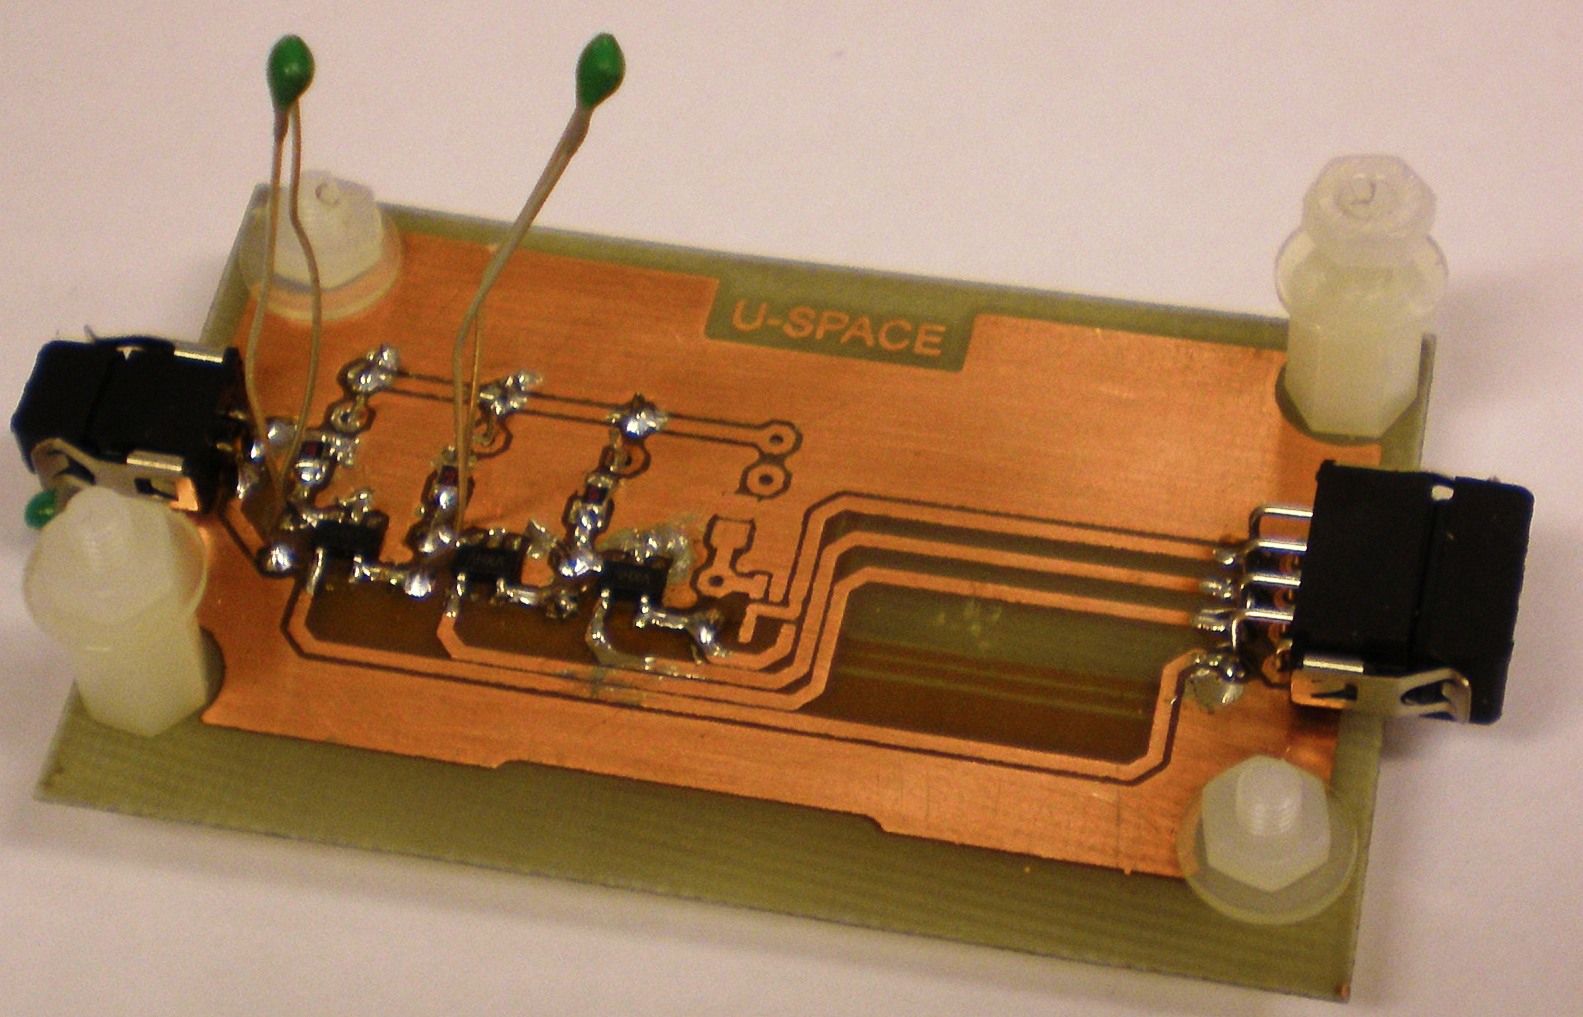
\includegraphics[width=0.7\textwidth]{figures/fig_Temp_top}
\caption{Temperature Sensor Board}
\label{fig:TS_top}
\end{figure}
%
\begin{figure}[H]
\centering
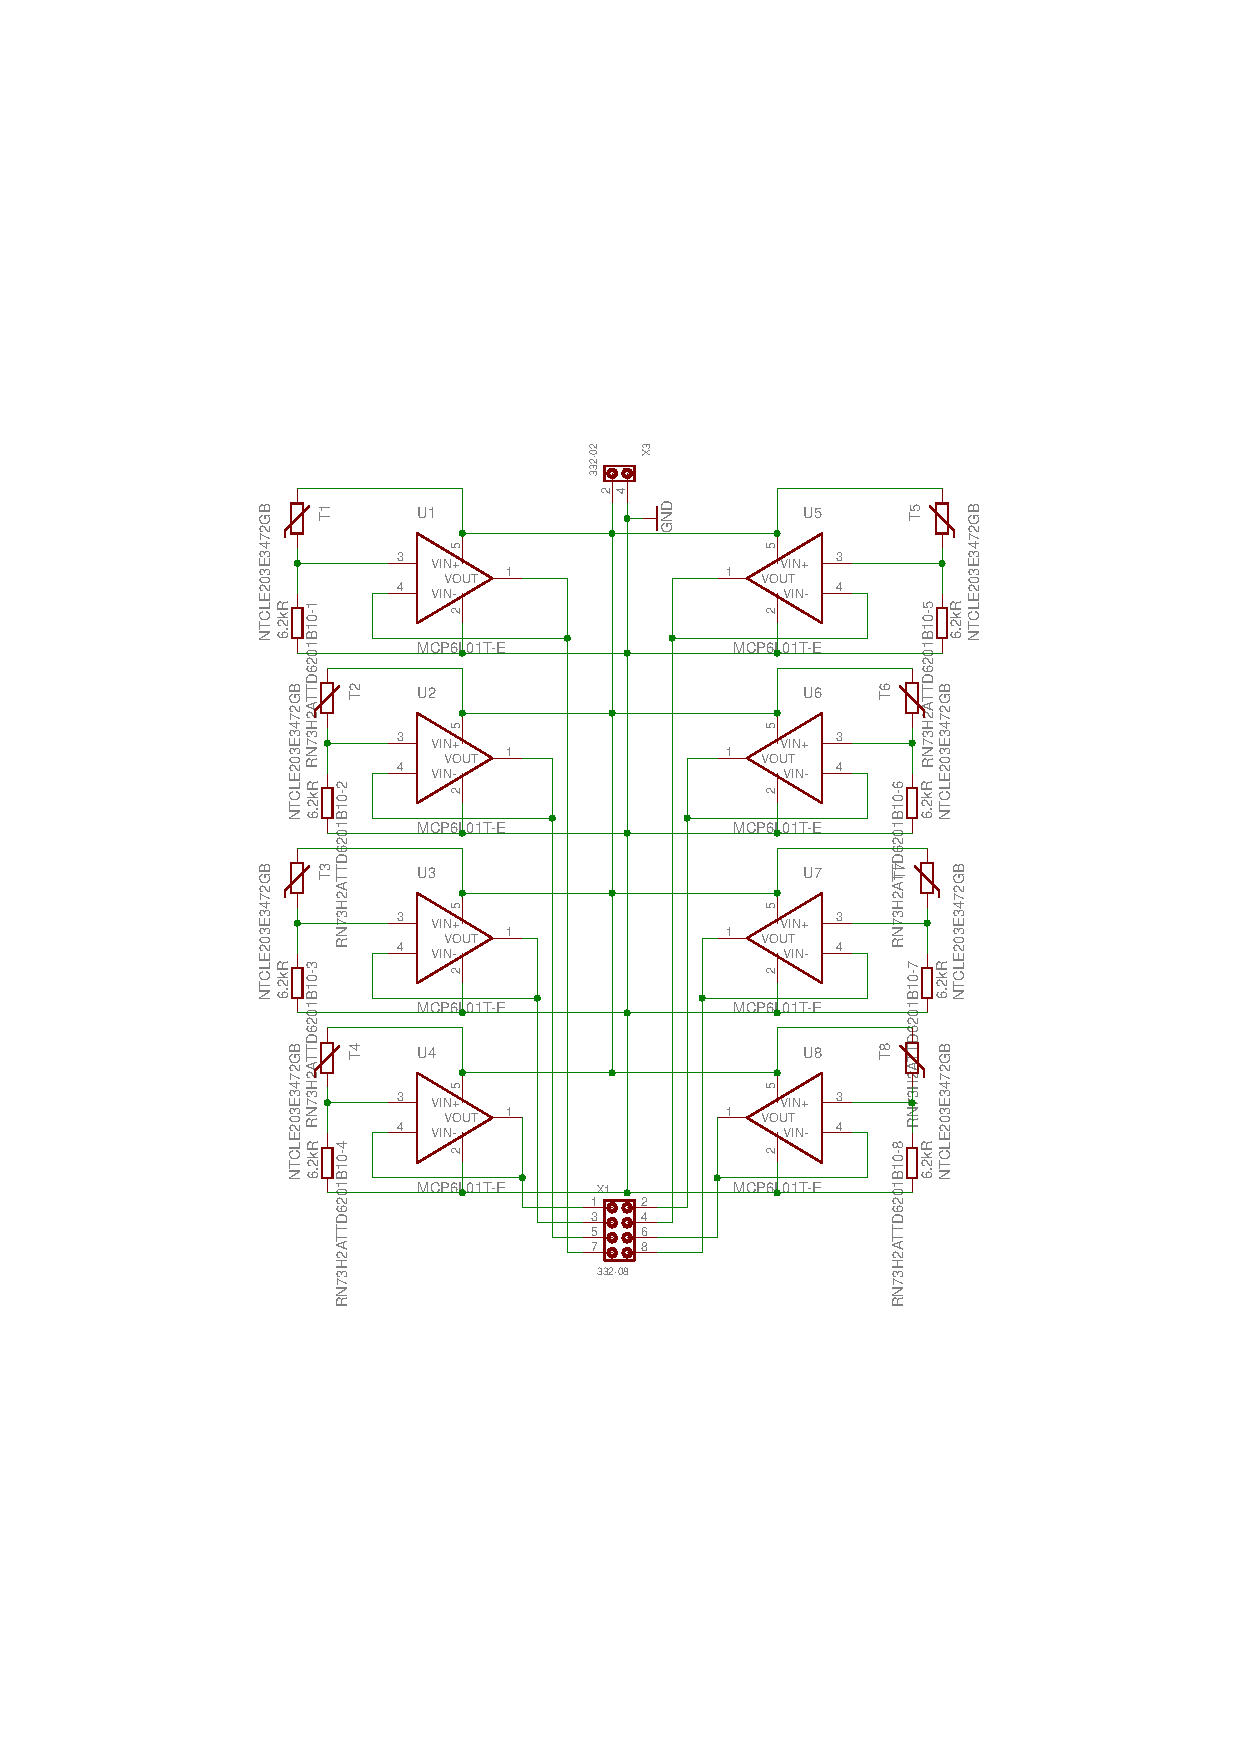
\includegraphics[width=\textwidth]{figures/fig_Schematic_TS}
\caption{Schematic of the Temperature Sensor Board}
\label{fig:Schematic_TS}
\end{figure}
%
%
\subsection*{Battery Handling}
%
%
During testing of a thermal design, one Li-ion battery underwent a heavy discharge and subsequently showed clear indication of damage (swelling of the battery pack). There was no immediate danger, however the incidence reminded us of the importance that everyone working with Li-ion batteries knows about its safe use and limitations. Li-ion fires are almost impossible to put out. Only useful method is to cover the battery in sand why we recommend LTU to put available a bucket of sand and/or establish a fire proof area/table for working with Li-ion batteries.
%
\section{Motor Control and Communication}
%responsible: Pedro and Morten
%
The only change in the \ac{MCC} was to re-program the flight controller such that it could operate two motors. 
%
%
%
 
\section{Imaging and Tracking Payload Unit}
\label{sec:changes_itpu}

In \cite{CDR} the \ac{ITPU} controller was illustrated using a RaspberryPi, but also as mentioned there, a \ac{BB} provides the processing capabilities and the interfaces in this project. In figure \ref{fig:itpu_setup}, the actual setup of the system is seen. Figure \ref{fig:itpu_pcb} shows the top and bottom view of the implemented \ac{PCB} which was designed to be tightly stacked to the main header of the BB and held in place by nylon screws.
%
\begin{figure}
\begin{centering}
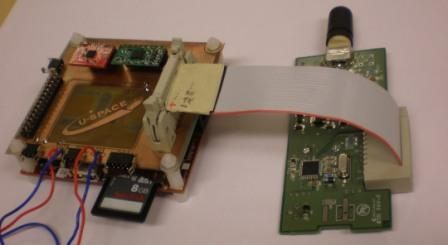
\includegraphics[height=0.25\textheight]{figures/itpu-setup.jpg}
\par\end{centering}
\caption{Setup of the ITPU consisting of the BeagleBoard, the E-Tag and the expansion board with sensors}
\label{fig:itpu_setup}
\end{figure}
%
%
\begin{figure}
\begin{centering}
\subfloat[Top]{\begin{centering}
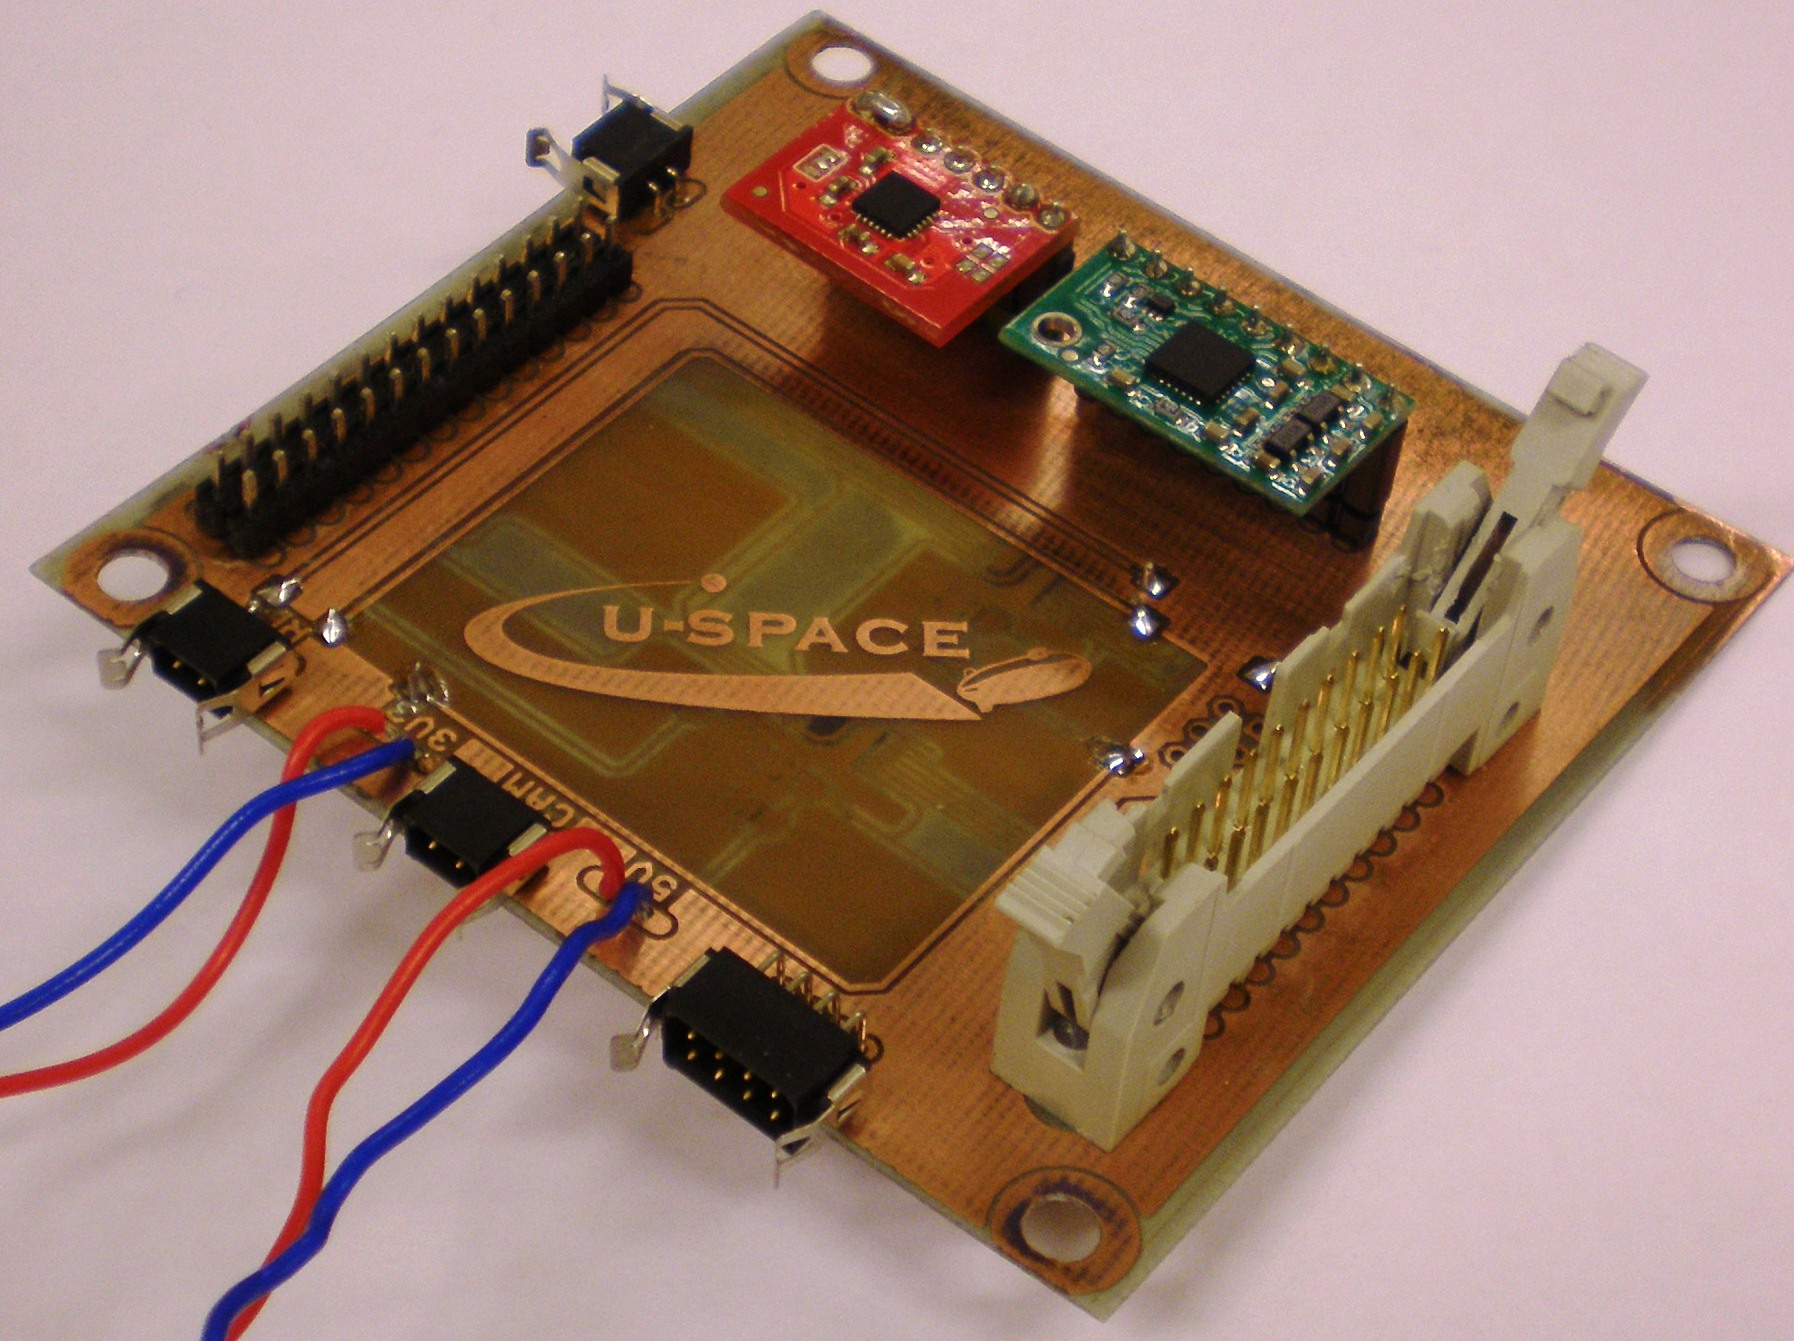
\includegraphics[height=0.25\textheight]{figures/LVC_top.JPG}
\par\end{centering}

}\subfloat[Bottom]{\begin{centering}
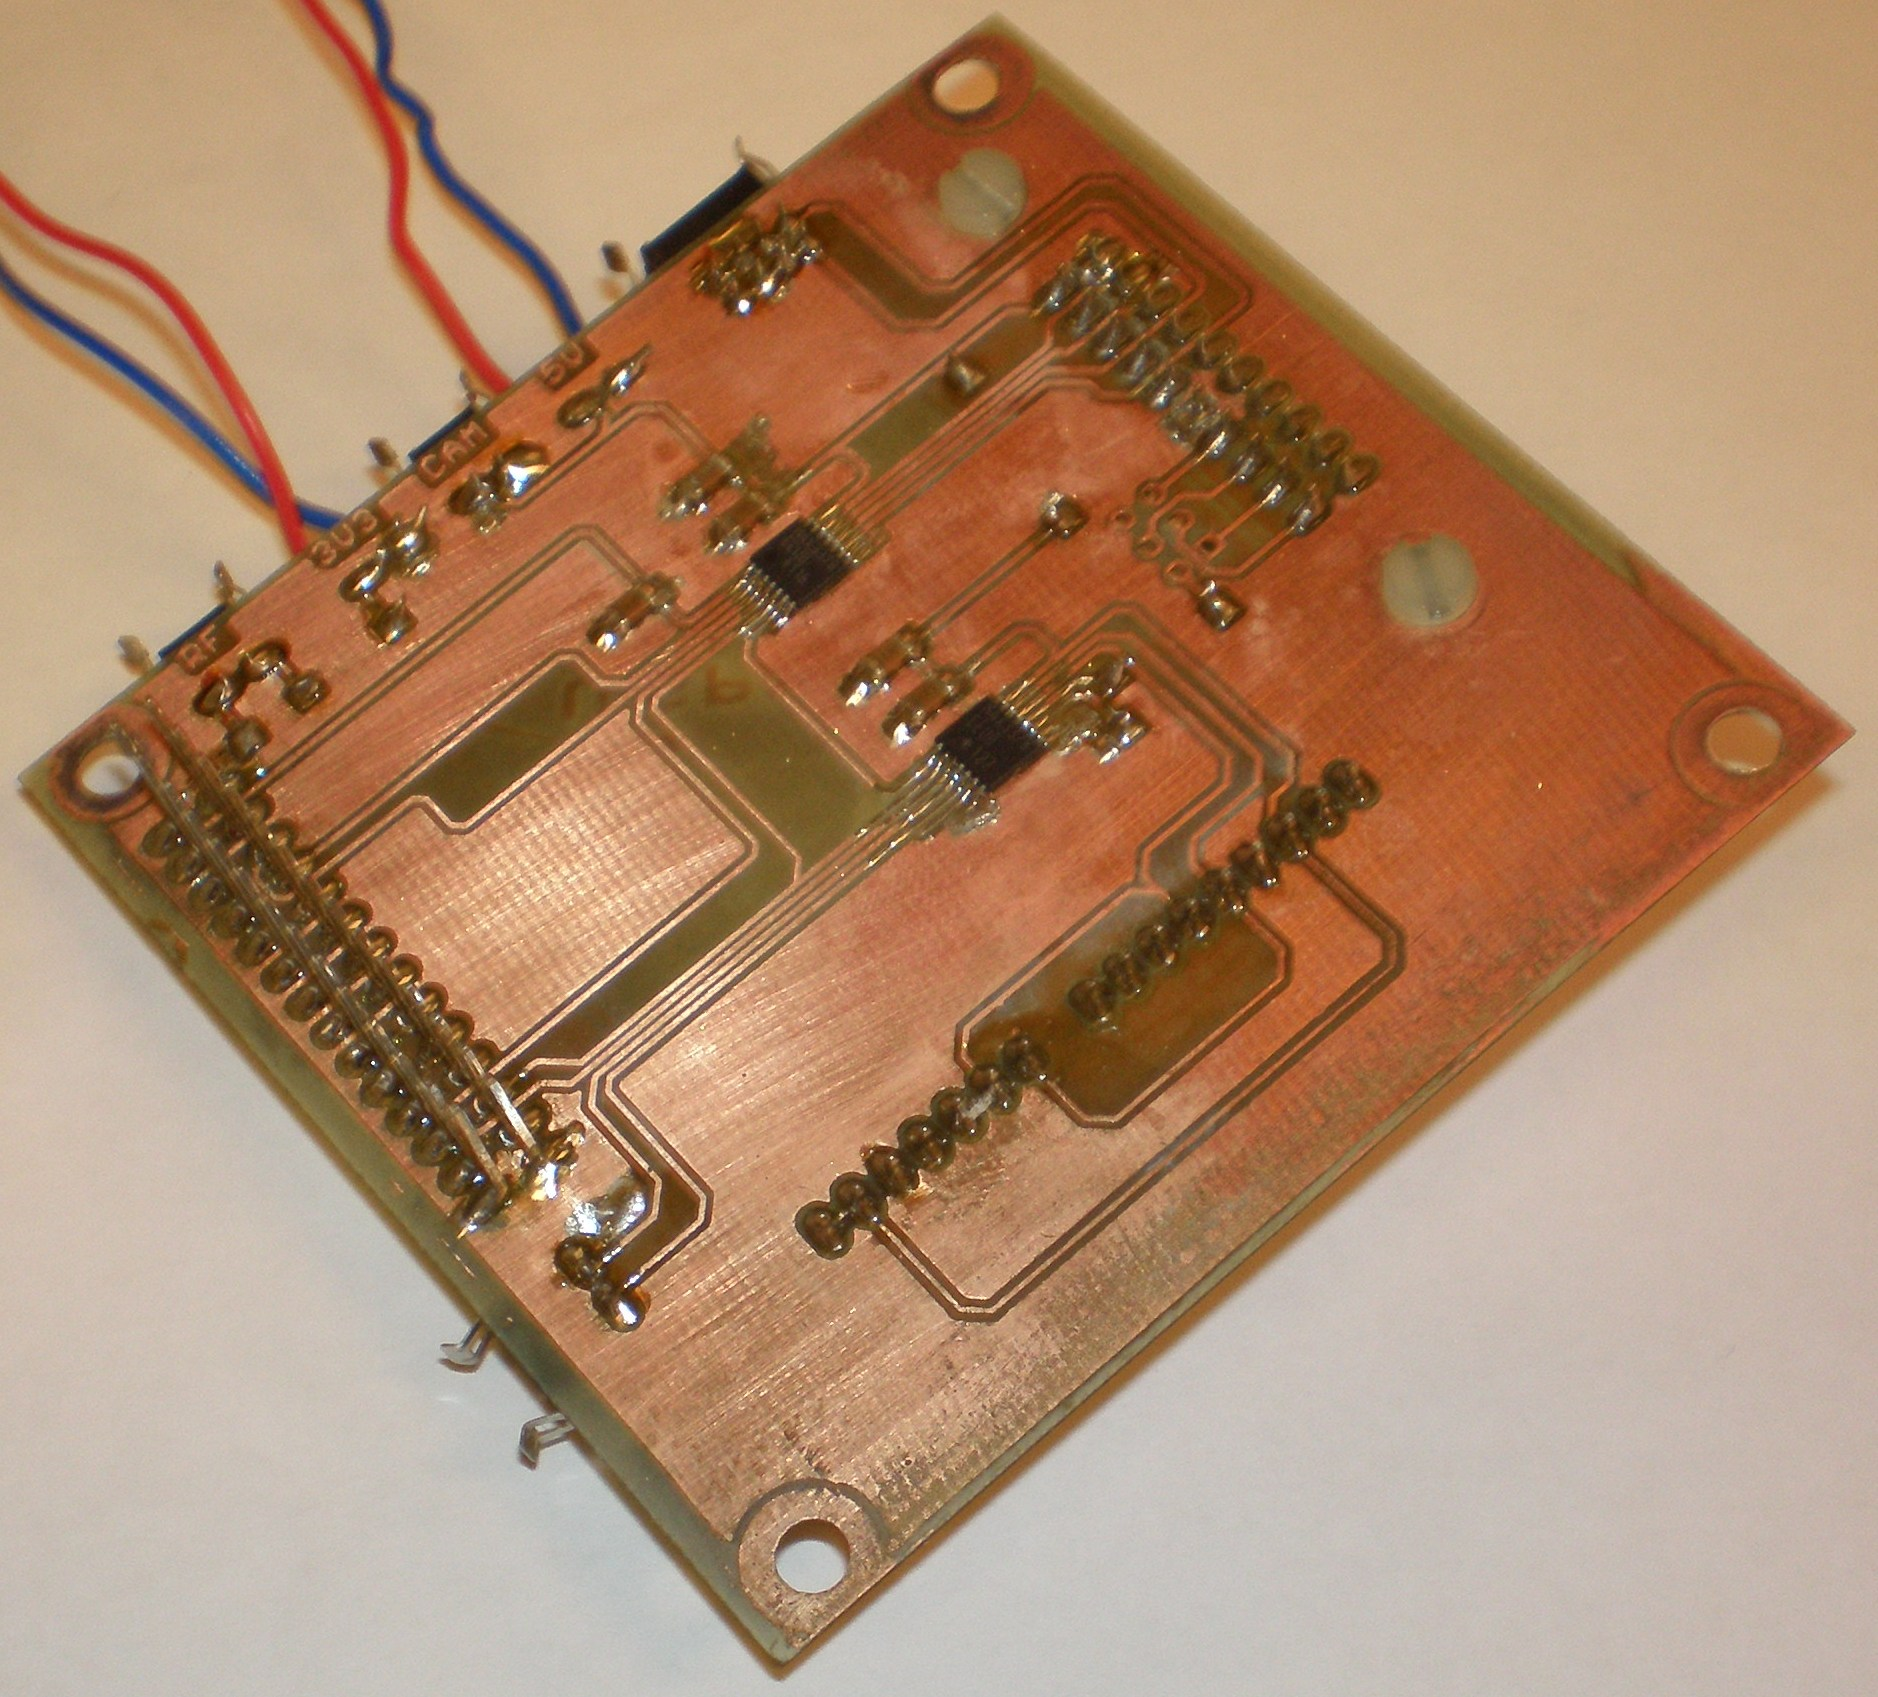
\includegraphics[height=0.25\textheight]{figures/LVC_bottom.JPG}
\par\end{centering}

}
\par\end{centering}
\caption{Populated expansion PCB of the ITPU}
\label{fig:itpu_pcb}
\end{figure}

Design changes were made to the ITPU circuit to include the communication and telemetry modules. The main expansion header of the \ac{BB} only provides access to one set of \ac{UART} pins which are used to communicate with the E-TAG GPS module. Another UART of the BB was muxed to the supplementary expansion header on J4, converted to a 3.3~V level and then connected to the X-Bee circuit board via wires. The \ac{I2C} interface was initially only planned to be converted from the 1.8~V level of the BB to the 3.3~V of the attitude sensors and vice versa. However, the telemetry conversion module (see \ref{sec:telemetryConv}) required a level shifter to 5~V for the ADCs. 

Both attitude sensor and telemetry system were stable when operating separately, but were unstable when operated in parallel on the same I2C-bus. As this was thought to be related to the multiple voltage level shifts, it was tried to use an additional I2C-bus muxed to pins J4 and J5 of the expansion header on the BB. However, the 2nd I2C-bus could not be activated on the BB rev.C4 used for the initial design.
On the software side, the integration of the telemetry and communication system together with the attitude determination and imaging system needed only minor additions to the code base to provide interfaces for communication between both systems. 

A major issue and cause for big changes compared to the CDR was the sudden failure of the BB between the pre-flight test and the scheduled flight-test. No replacement board of the same kind could be acquired on such a short notice so a provided BB-xM was made to fit into the already designed and build system. Although the BB-xM is in general pin-compatible to the BB rev.C4, a problem was the direction of the main expansion header. In the initial BB, the female-header was mounted on the top side of the BB, hence the ITPU-PCB was designed to directly stack on top of the BB. The expansion header of the BB-xM was mounted to the bottom side. Therefore, a direct connection between the two boards was no longer possible. Instead, ribbon cable had to be produced however this could not provide a fully stable connection between the BB-xM and the expansion board. However on the BB-xM it was possible to enable the second I2C-bus on the J4 and J5 expansion headers.

%responsible: Jan

\section{Communication Subsystem}
\label{sec:com}
%responsible: Omair
There is no change in the design of the \ac{TTC} subsystem from the CDR report \cite{CDR_TTC}. The \ac{U-SPACE} communication protocol was implemented in C language for the on-board computer (Beagle board) and the ground station in LabView, due to its nice graphical environment. A custom \ac{PCB} was designed and developed for the conversion of analogue \acp{TM}. A second \ac{PCB} was designed for housing and interfacing of the Xbee radio with the \ac{BB}. \ac{TTC} or communication subsystem provided the interface between the \ac{U-SPACE} and the ground station. This wireless connection is shown in figure \ref{fig:com_setup}. According to the test and verification plan in \cite{CDR_TTC}, testing of the on-board software and the ground station was successfully executed.
%
\begin{figure}[bht]
\centering
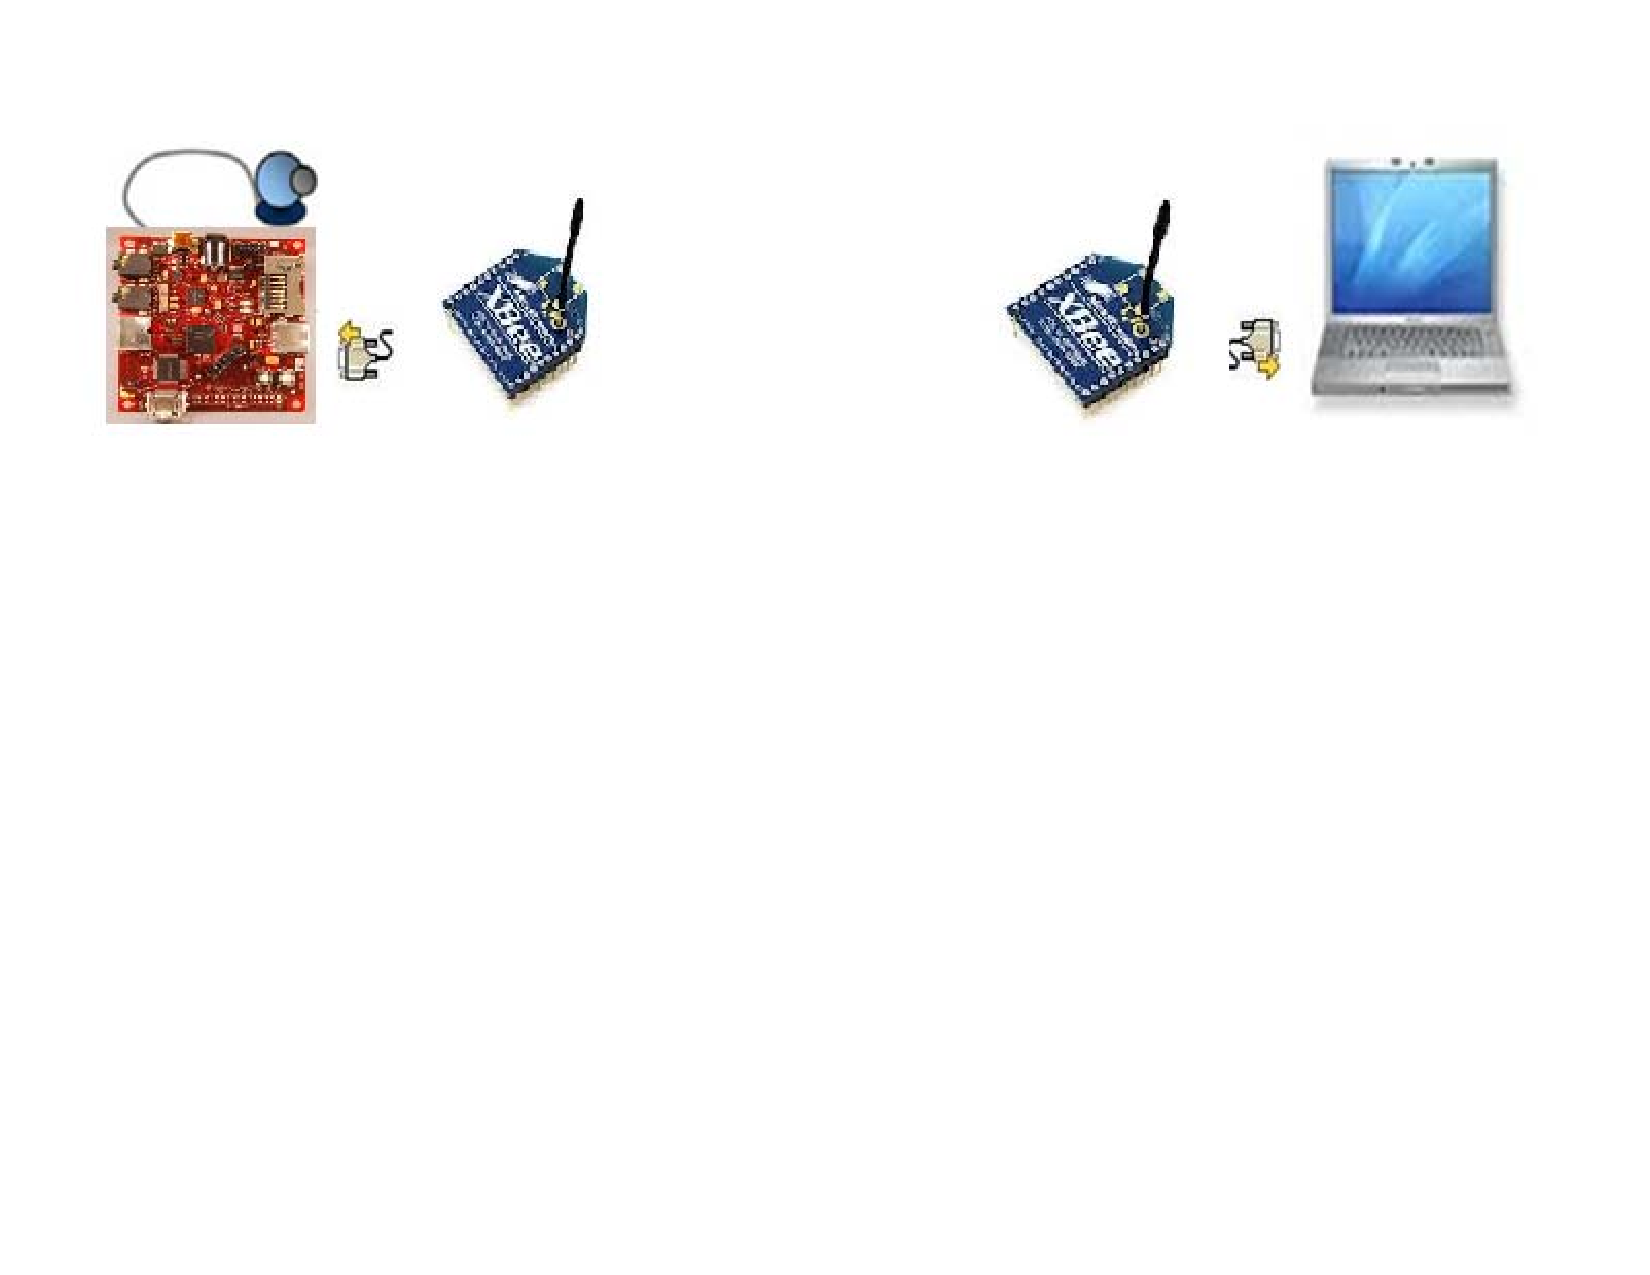
\includegraphics[width=\textwidth]{figures/com_setup.pdf}
\caption[\ac{U-SPACE}Communication overview]{\ac{U-SPACE} Communication overview}
\label{fig:com_setup}
\end{figure}
%
\subsection{Telemetry}
\label{Number_of_telemetries}
The \ac{U-SPACE} protocol is divided into subsystems according to different functionalities. All important parameters of each subsystem, which need to be monitored on the ground station, are considered as telemetry. Telemetry implementation details are given in table \ref{tab:telemetry_uspace}. \ac{U-SPACE} has synchronization value ``$0\text{x}0C$''. Power subsystem has ID $0\text{x}11$. This subsystem ID is followed by one byte parameter ID. Both subsystem ID and parameter ID makes a unique identifier, TM ID. Data size for all power telemetries is $10$ bytes(char). \ac{OBDH} subsystem ID is $ 0\text{x}33 $ and size of $10$ bytes for all telemetries. \ac{ADCS} subsystem ID is $0\text{x}55$ and contains only one telemetry which is the attitude information. This attitude data contains all three rotation angles in a single packet of $30$ byte data size. The GPS subsystem ID is $ 0\text{x}77 $ and contains three telemetries; latitude, longitude and altitude. Data size of each GPS telemetry is $10$ bytes.

\begin{table}[bht]
\centering
\caption[Telemetry list of the U-SPACE]{Telemetry list of \ac{U-SPACE}}
\label{tab:telemetry_uspace}
%\rowcolors{3}{tableshade}{white}
\begin{tabular}{|m{0.15\textwidth}m{0.1\textwidth}m{0.15\textwidth}m{0.1\textwidth}m{0.4\textwidth}|}
\hline
\textbf{Subsystem}		&  		\textbf{TM ID}				&	\textbf{size(char)}			&	\textbf{Type}& 		\textbf{Description}  			  \\ 
\hline\hline
\multirow{11}{*}{Power} &    $ 0\text{x}1141 $				&	$ 15 $						&    Analogue    &    	Under Voltage Lock-Out Status     \\
						&    $ 0\text{x}1142 $				& 	$ 15 $						& 	 Analogue	 &	 	Voltage of LiPo battery cell 2    \\
						&    $ 0\text{x}1143 $				&   $ 15 $						& 	 Analogue	 &	 	Battery discharge current  		  \\
						&    $ 0\text{x}1144 $				& 	$ 15 $						&	 Analogue	 &		Voltage of LiPo battery cell 1    \\
						&    $ 0\text{x}1145 $				& 	$ 15 $						&	 Analogue	 &		Temperature of battery  	  	  \\
						&    $ 0\text{x}1146 $				&   $ 15 $						&	 Analogue	 &		Charge controller status  	 	  \\
						&    $ 0\text{x}1147 $				&   $ 15 $						&	 Analogue	 &		Battery charge current  	  	  \\
						&    $ 0\text{x}1148 $				&   $ 15 $						&	 Analogue	 &		3.3V supply current  		 	  \\
						&    $ 0\text{x}1149 $				&   $ 15 $						&	 Analogue	 &		3.3V supply voltage  		      \\
						&    $ 0\text{x}114A $				&   $ 15 $						&	 Analogue	 &		5.0V supply current 	    	  \\
						&    $ 0\text{x}114B $				&   $ 15 $						&	 Analogue	 &		5.0V supply voltage  		 	  \\
\hline
\multirow{5}{*}{OBDH}   &    $ 0\text{x}3351 $				&	$ 15 $						&	 Analogue	 &      Temperature Motor 1			      \\
						&    $ 0\text{x}3352 $				&	$ 15 $						&	 Analogue	 &      Temperature Motor 2	   		      \\
						&    $ 0\text{x}3353 $				&	$ 15 $						&	 Analogue	 &      Temperature Atmosphere		      \\
						&    $ 0\text{x}3354 $				&	$ 15 $						&	 Analogue	 &      Temperature Electronics Bay	      \\
						&	 $ 0\text{x}3355 $				&	$ 35 $						&	 Digital	 &      UTC Time					      \\
\hline
\multirow{1}{*}{ADCS}   &    $ 0\text{x}5561 $ 				&	$ 35 $						&	 Digital	 &	    Roll, Yaw and Pitch	       		  \\
\hline
\multirow{3}{*}{GPS}    &    $ 0\text{x}7771 $				&	$ 15 $						&	 Digital	 &      Latitude		       	    	  \\
						&    $ 0\text{x}7772 $				&	$ 15 $						&	 Digital	 &      Longitude	   				      \\
						&    $ 0\text{x}7773 $				&	$ 15 $						&    Digital	 &      Altitude  				          \\ 
\hline
\end{tabular}
\end{table}
%

\subsection{Telecommands}
\label{subsec:telecommand}
Table \ref{tab:telecommand_uspace} lists all implemented telecommands. Telecommands can be sent to configure the on-board computer for different modes of telemetry or configure a specific subsystem. There are six different modes of the telemetry which are listed in table \ref{tab:TM_modes} along with the data rate for each mode. All telecommands are implemented under the \ac{OBDH} subsystem. Details of implementation according to the telecommad format are given in table \ref{tab:telecommand_uspace}.
%
\begin{table}[bht]
\centering
\caption[Data rate for different \ac{TM} modes]{Data rate for different \ac{TM} modes}
\label{tab:TM_modes}
%\rowcolors{3}{tableshade}{white}
\begin{tabular}{|m{0.4\textwidth}m{0.4\textwidth}|}
\hline
\textbf{TM mode}			&  		\textbf{Data rate(bps)}   \\
\hline
Switch off telemetries		&		$ 0 $		 			  \\
Power only	   		        &		$ 1320 $		 		  \\
\ac{OBDH} only	      	  	&		$ 760 $		 			  \\
ADCS only			      	&		$ 280 $		 			  \\
GPS only		   		    & 		$ 360 $		 			  \\
All telemetries	      	  	&		$ 2720 $		 		  \\
\hline
\end{tabular}
\end{table}
%
%
Three telecommands are implemented for the payload (camera). Camera set command is implemented to set the time interval between two successive images. After setting the image interval, camera start command is used to instruct the on-board computer to take picture after the specified time interval. Third is the camera stop command which will stop the camera. In future, if real time \ac{PWM} control is implemented, commands for speed control of the motor can be incorporated. Then, the use of the flight control joystick can be discarded and everything fully controlled via the Xbee radio link.

\begin{table}[bht]
\centering
\caption[Telecommand list of the U-SPACE]{Telecommands of \ac{U-SPACE}}
\label{tab:telecommand_uspace}
%\rowcolors{3}{tableshade}{white}
\begin{tabular}{|m{0.15\textwidth}m{0.1\textwidth}m{0.15\textwidth}m{0.2\textwidth}m{0.25\textwidth}|}
\hline
\textbf{Subsystem}		&  		\textbf{TM ID}				&	\textbf{size(char)}		&	\textbf{Data field}	& 		\textbf{Description}  	  \\ 
\hline\hline
\multirow{9}{*}{OBDH}   &    $ 0\text{x}33B2 $				&	$ 16 $					&	image interval		&      Camera Set			      \\
						&    $ 0\text{x}33B3 $				&	$ 16 $					&	$ 0\text{x}00 $		&      Camera Start	   		      \\
						&    $ 0\text{x}33B4 $				&	$ 16 $					&	$ 0\text{x}00 $		&      Camera Stop		      	  \\
						&    $ 0\text{x}33B1 $				&	$ 16 $					&	$ 0\text{x}00 $		&      Switch off telemetries	  \\
						&    $ 0\text{x}33B1 $				&	$ 16 $					&	$ 0\text{x}10 $		&      Power only	   		      \\
						&    $ 0\text{x}33B1 $				&	$ 16 $					&	$ 0\text{x}20 $		&      \ac{OBDH} only	      	  \\
						&    $ 0\text{x}33B1 $				&	$ 16 $					&	$ 0\text{x}40 $		&      ADCS only			      \\
						&    $ 0\text{x}33B1 $				&	$ 16 $					&	$ 0\text{x}50 $		&      GPS only		   		      \\
						&    $ 0\text{x}33B1 $				&	$ 16 $					&	$ 0\text{x}70 $		&      All telemetries	      	  \\
\hline
\end{tabular}
\end{table}
\subsection{Telemetry Conversion Module}
\label{sec:telemetryConv}
%
Telemetry Type in table \ref{tab:telemetry_uspace} is stated analogue if the sensor does not have a built-in \ac{ADC} and requires an external \ac{ADC} for on-board processing. The \ac{BB} does not include \ac{ADC}. Instead, a custom \ac{PCB} has been designed and implemented which is capable of converting all analogue telemetries from table \ref{tab:telemetry_uspace} into digital domain. The conversion module includes two ADC AD7998 chips  from Analog Devices. AD7998 is a 12 bit \ac{ADC} chip with eight input channels and a multiplexer on a single IC. Diodes are added to protect the inputs from high voltages exceeding 5 V. A second PCB has been designed for housing the on-board X-bee Pro. This \ac{PCB} will interface the Xbee pro module to 
the \ac{BB} for transmission and reception of the telecommands and telemetries.\\
%
\begin{figure}[bht]
\centering
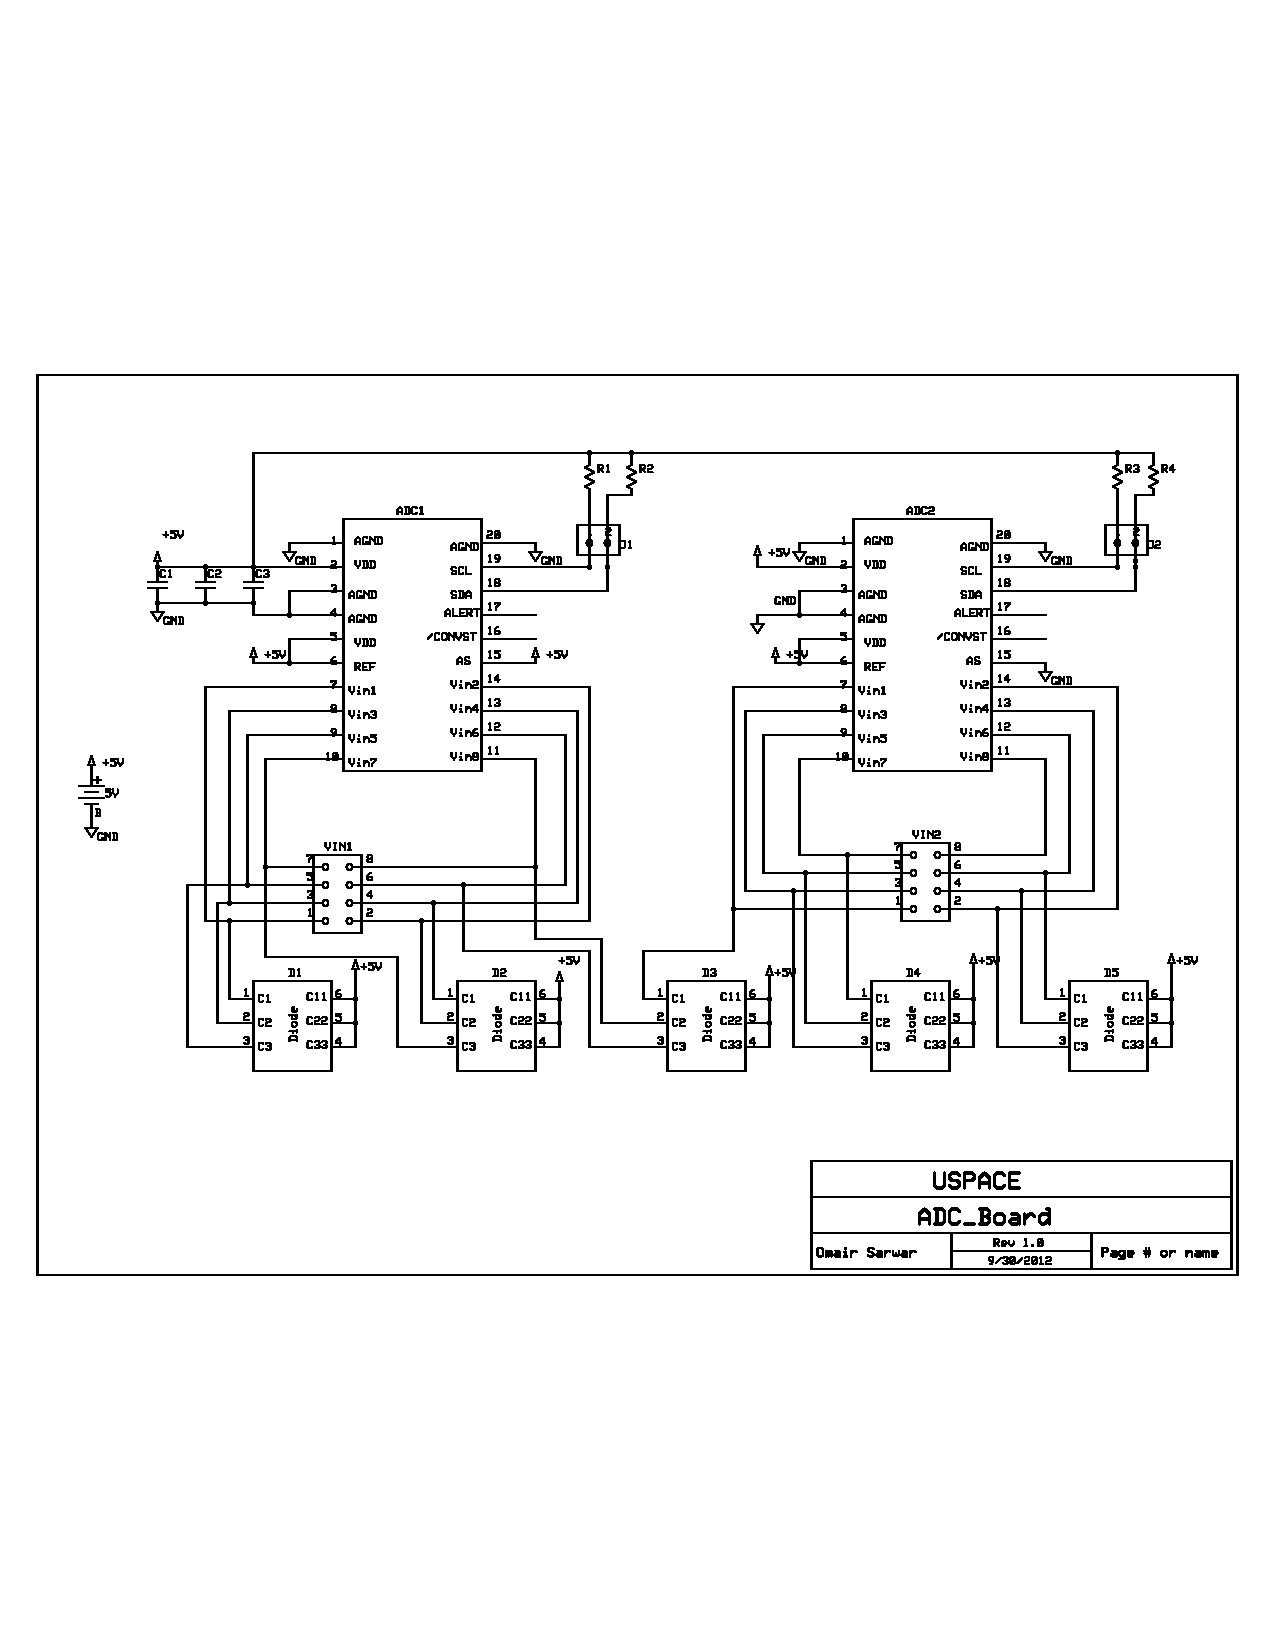
\includegraphics[scale=0.7]{figures/schematic_conversion_module.pdf}
\caption{Schematic of telemetry conversion module}
\label{fig:schematic_conversion_module}
\end{figure}

\begin{figure}[bht]
\centering
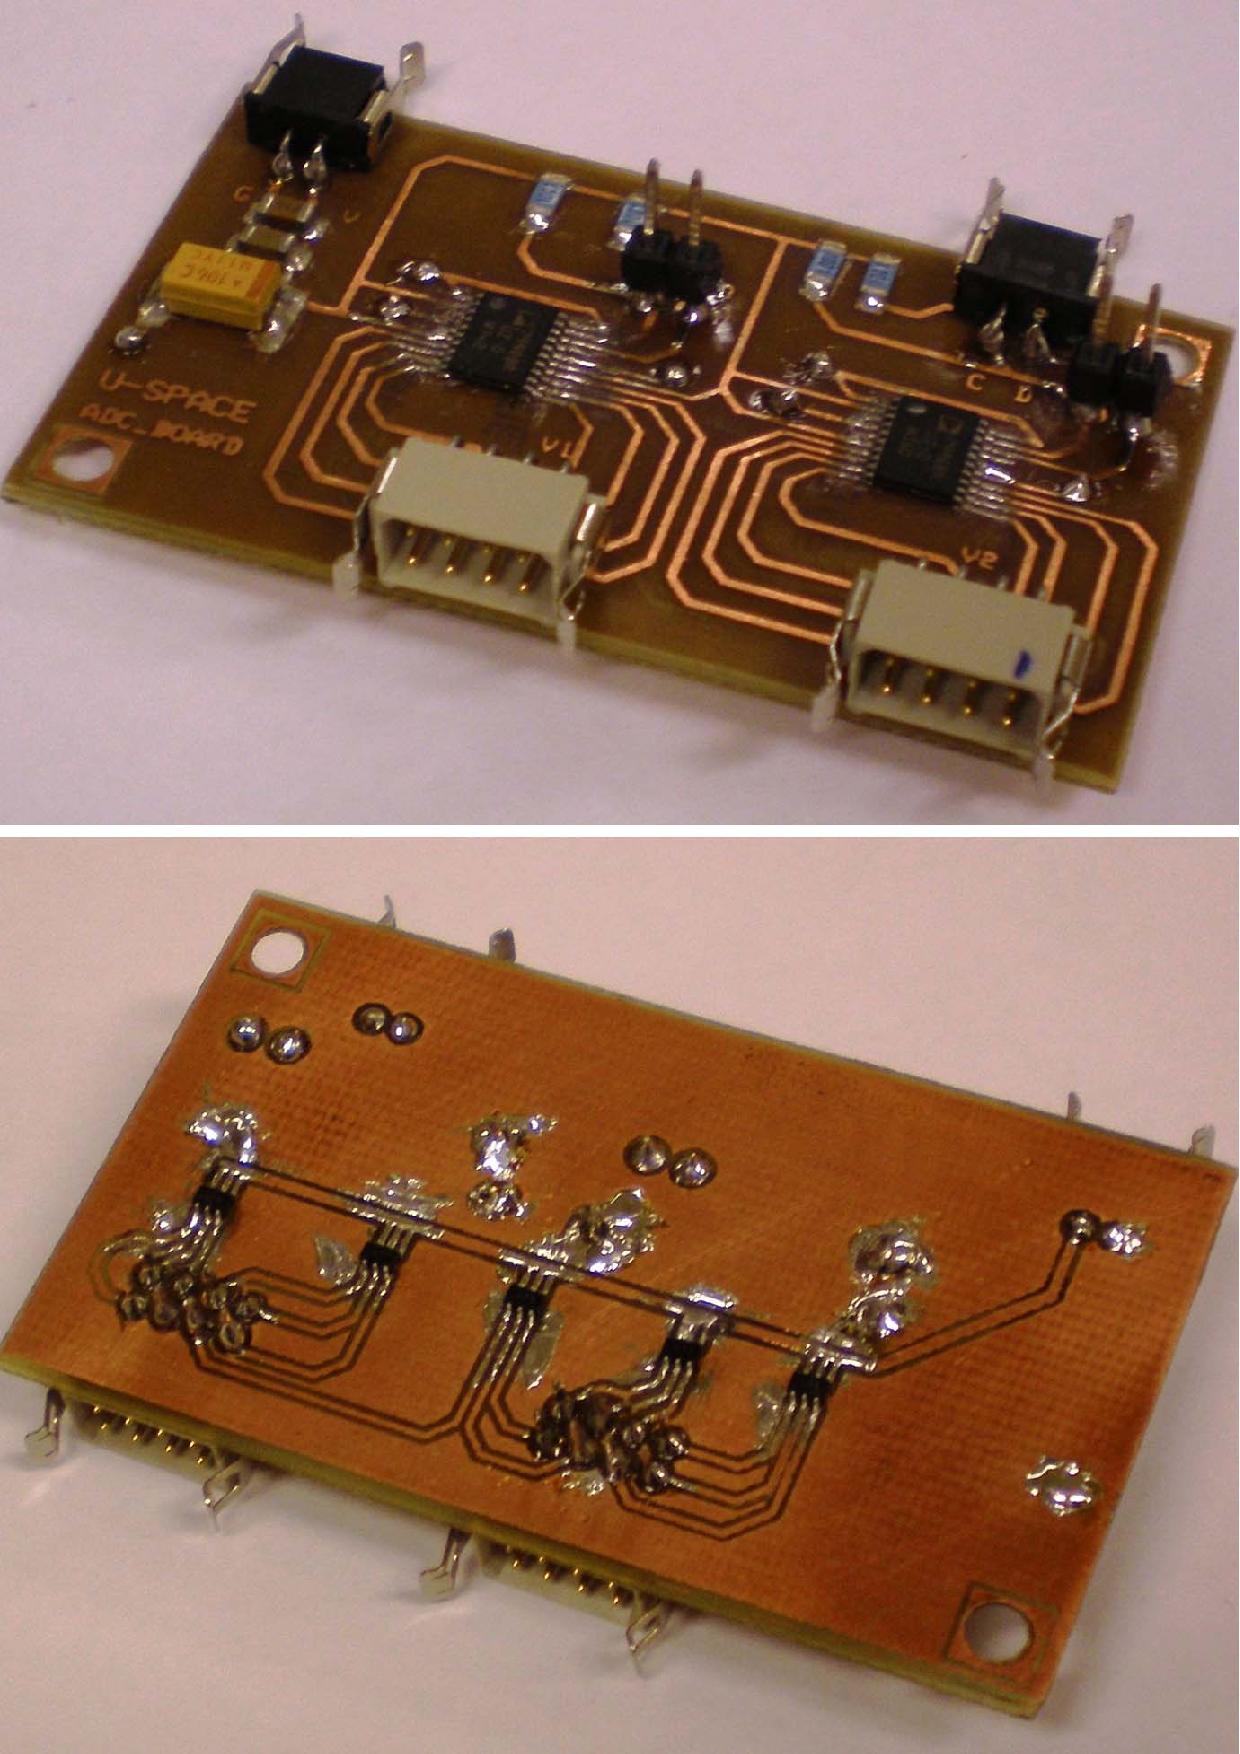
\includegraphics[scale=0.45]{figures/PCB_conversion_module.pdf}
\caption{\ac{PCB} of Conversion module}
\label{fig:PCB_conversion_module}
\end{figure}
%
Interfacing of the conversion module with the \ac{BB} is shown in figure \ref{fig:conversion_module}. AD7998 provides data and channel ID on a $5$ V I$2$C bus which connects to the BB I$2$C bus. However, the \ac{BB} I$2$C bus is at $1.8$ V so a level converter has been developed (refer \cite{CDR}) to convert the $5.0$ V and $3.3$ V I$2$C bus to a $1.8$ V I$2$C bus.
%
\begin{figure}[bht]
\centering
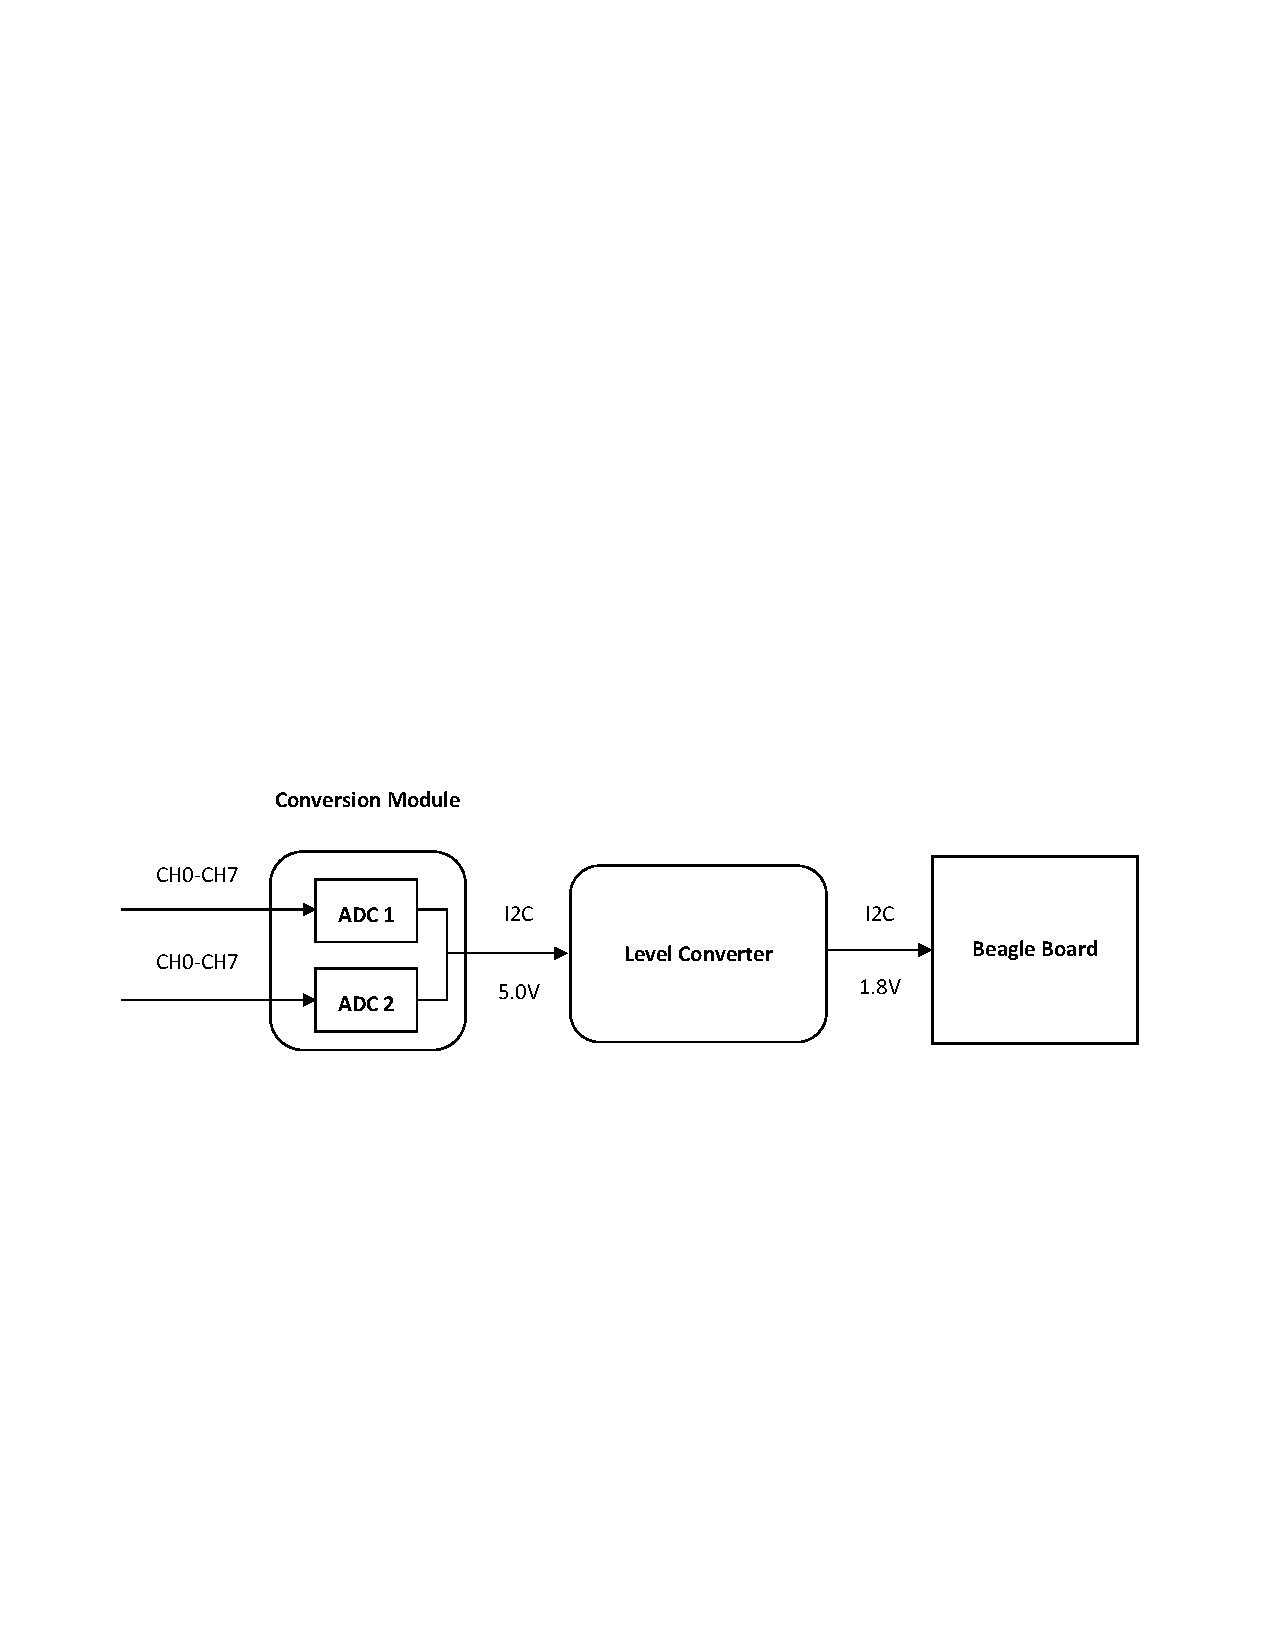
\includegraphics[scale=0.7]{figures/conversion_module.pdf}
\caption{Conversion module interface with Beagle board}
\label{fig:conversion_module}
\end{figure}
%
%
\subsection{U-SPACE Ground Station}
The ground station is implemented in LabView. The front panel view of the \ac{U-SPACE} ground station is shown in figure \ref{fig:Labview_ground_station}. The following section, describes how to use the ground station. A serial link is established between the computer running the LabView ground station and the Xbee radio. The ''COM'' section configures this serial link. Here, the data rate, parity bit, start and stop bit can be set. These parameters should be the same as configured for the on-board computer. There is also a ``Debug'' window which displays the serial communication data for debugging purposes. \\
%
For generating telecommands, there is one section on the upper left part of the front panel of the ground station. First, the subsystem to receive the telecommand is selected. This will select the subsystem ID. Then the property (parameter) to configure is selected thus setting of the subsystem property ID is done. Finally, data field is filled with the appropriate value in accordance to on-board computer software. Clicking the ``SEND'' button generates the telecommand and sends it via the Xbee radio. The concatenated telecommand according to \ac{U-SPACE} communication format can be shown in the ``Debug'' window. A separate telecommand section is also dedicated to configure the \ac{U-SPACE} telemtry modes as described in section \ref{subsec:telecommand}. Select the mode from the drop down menu and click ``SEND TM'' button.
\\
  %
\begin{figure}[bht]
\centering
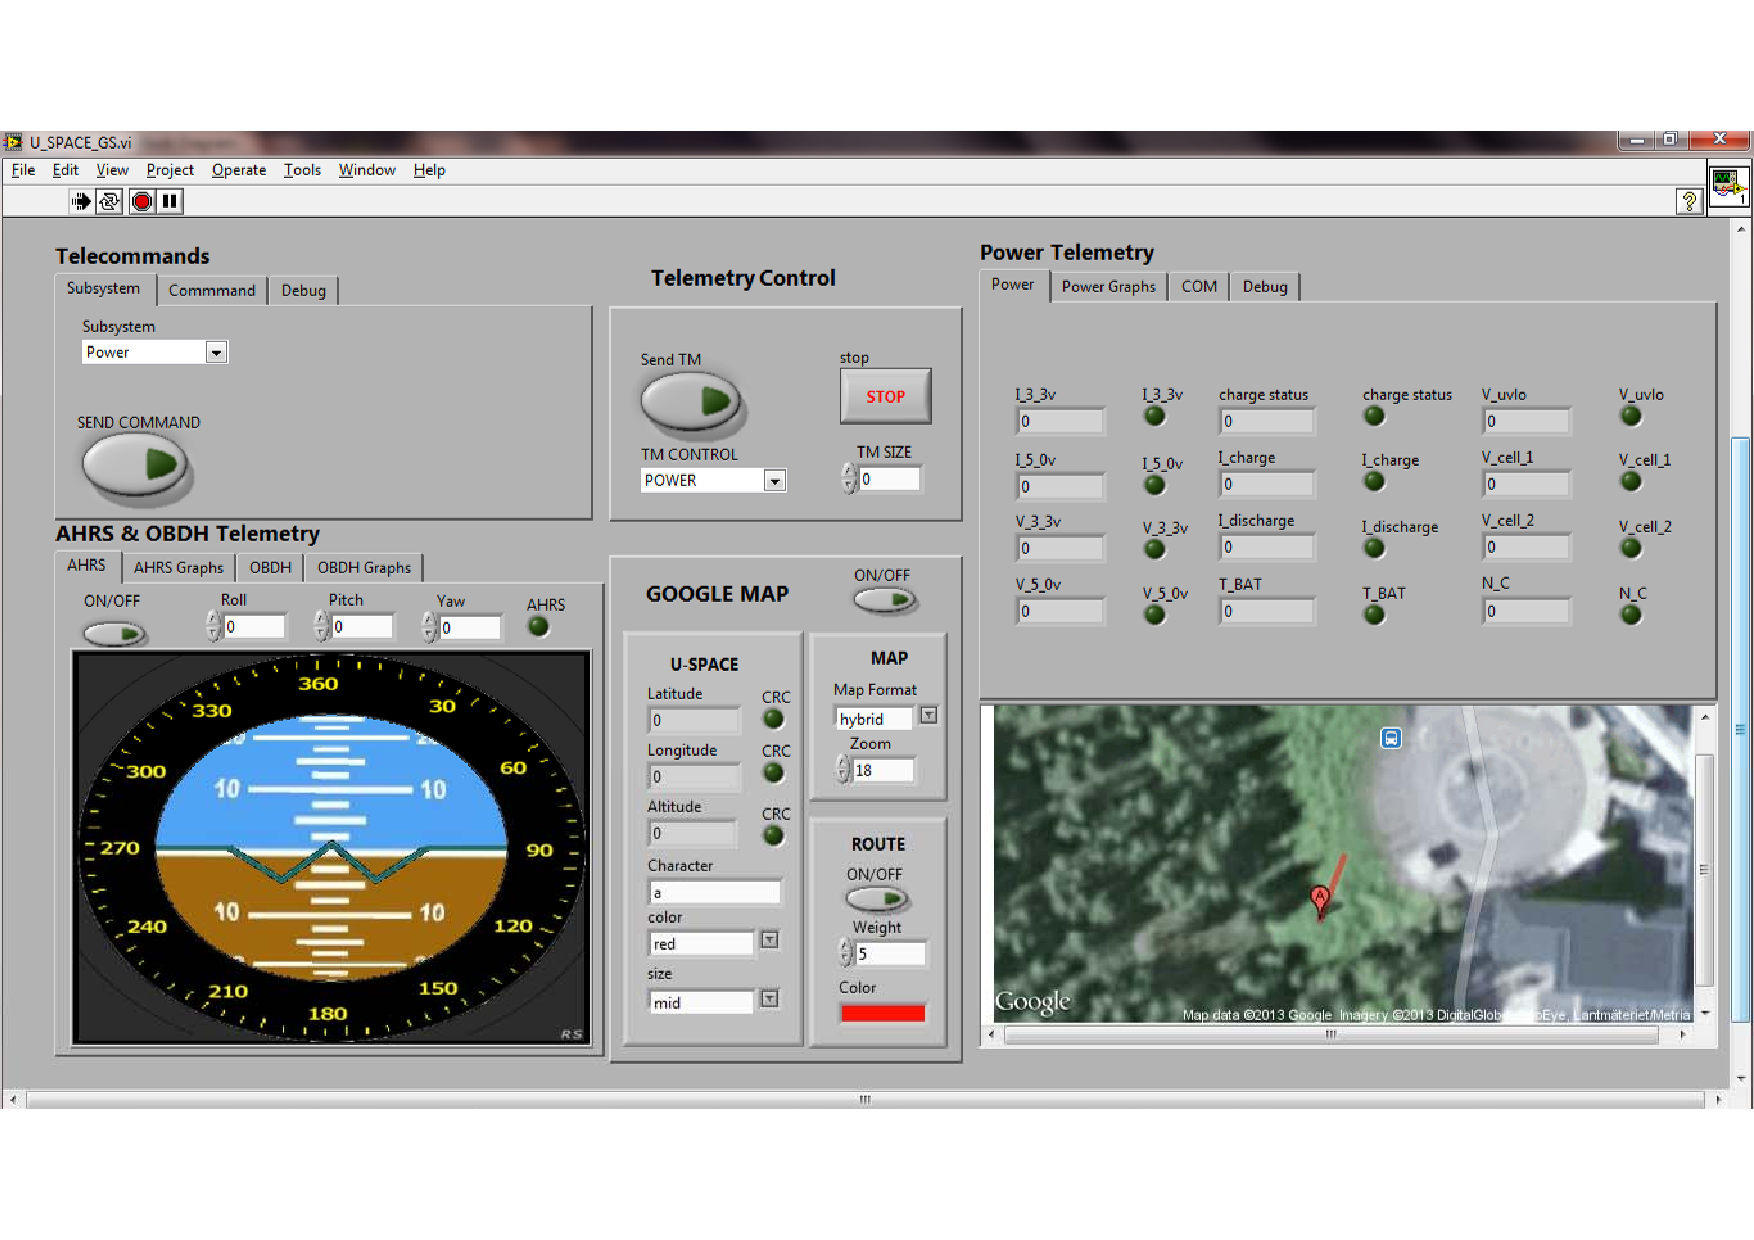
\includegraphics[scale=0.5]{figures/GS.pdf}
\caption{U-SPACE ground station Lab View Front Panel}
\label{fig:Labview_ground_station}
\end{figure}
%
On the front panel of the ground station, telemetries are displayed in groups according to the subsystem. Power telemetries are on the upper right corner. All eleven telemetries are displayed numerically. There are three telemetries in the power graphical display; battery voltage, battery current and discharge current. To see the graphical display, go to ``Power graphs'' and then select the telemetry for graphical display from drop down menu.\\ 
\ac{ADCS} and \ac{OBDH} telemetries are shown in left lower corner. \ac{ADCS} contains three attitude parametrs; roll, pitch and yaw in numerical display. To display these on the artificial horizon, click the ON/OFF button. Artificial horizon consists of three images: roll, pitch and heading respectively. They move according to attitude input data. All \ac{OBDH} telemetries are displayed numerically in a separate window which is embedded with the \ac{ADCS} subsystem. However, four \ac{OBDH} temperatures: ambient, cargo bay and one of each motor are also displayed in the ``\ac{OBDH} graph window'' Here is also displayed the temperature change rate during different flight phases.\\
%
\noindent
For the GPS subsystem, telemetries are shown in numerically in the right lower corner of the front panel view of the ground station. To show the position on Google Maps, an internet connection is required. This is a static image implementation of the desired latitude, longitude, image size and the resolution. Select the \ac{U-SPACE} indicator parameters: character (showing \ac{U-SPACE}), colour and font for display. Also select the type of map and click the Google Maps ``ON/OFF'' button. This will generate an \ac{URL} according to the selected characteristics and will download the corresponding static image from Google Maps. To show the route from the starting point, select route characteristics and click show route ``ON/OFF button''. This will track the \ac{U-SPACE} from the starting point.

\subsection{Electrical Connectors Layout}
Figure \ref{fig:Electrical_Connections} shows the electrical connections on block diagram of the complete U-SPACE system.
%
\begin{figure}[h!]
\centering
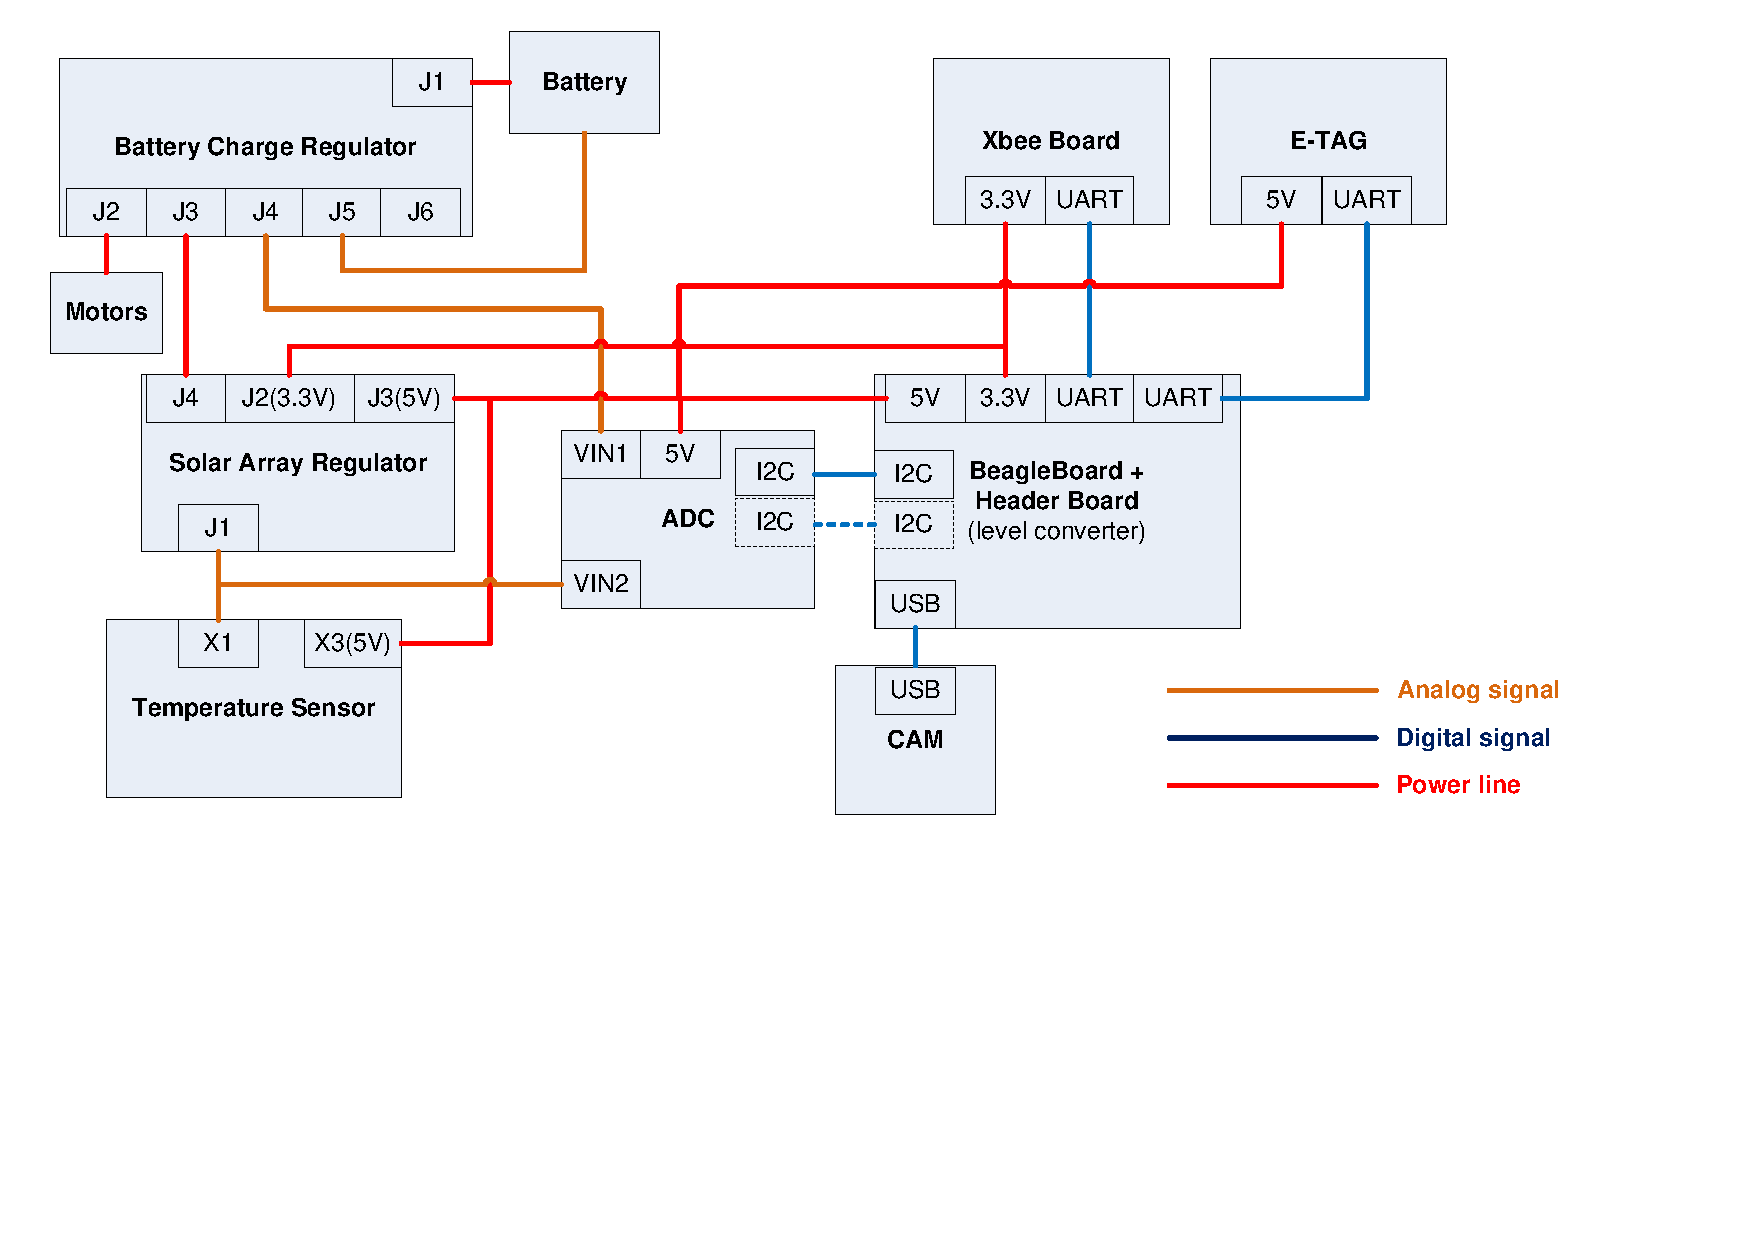
\includegraphics[width=\textwidth]{figures/fig_Electrical_Connections_Layout}
\caption{Electrical connectors layout}
\label{fig:Electrical_Connections}
\end{figure}


\section{Mechanical Structure and Envelope}
%responsible: Pedro 

The following section discusses changes made to the \ac{MSE}. The envelope has not suffered any modifications since it is the same Esrange blimp presented in the CDR and modifications to it were not possible. On the other hand, the payload box presented in the CDR was discarded and a new one designed. 

\subsection{Cargo Bay}
After the summer break we reached the conclusion that the old payload box was not rigid enough to withstand any moderate compression/traction load or unexpected shock loads, i.e. dropping the box or a sudden landing when already attached to the blimp.  Since we needed to increase the strength of the structure and at the same time keep it low weight, we decided to build the frame out of hollow carbon fiber rods with a squared section. To join them, an epoxy glue was used. 
The final result showed an enhanced structural strength compared with the first cargo bay frame. To further reinforce the frame, we decided to build aluminium corner pieces that at the same time served as a support for the thermal insulating walls, the cargo bay top plate connecting the motor rod and the bottom plate housing the electronics. The final design for the payload box can be summarized as follows:

\begin{itemize}
\item Rigid carbon fiber frame.
\item 8 aluminum corner pieces + 3x8 bolts to fasten each corner
\item 6 Styrofoam insulating walls
\item Payload surface to house the electronics
\item Roof section, including the clamps to hold the rod of the motors
\item 4 clamps at the bottom of the box as support legs
\end{itemize}

\section{Thermal Design}
A thermal insulation is needed in order to keep the payload components within their allowed working temperature ranges. To achieve this, 6 different Styrofoam walls were designed to cover the carbon fiber frame. The walls where cut with the hot wire with a 5 mm thickness and the corresponding dimensions for each wall. 
The thickness was chosen after an extensive series of experiments and tests to determine the right value that would be able to keep the payload within the expected range of temperatures. The critical component of the payload is the Li-ion battery since it has a much more restricted working temperature range than the electronics. This element constrained the temperature inside the payload box to be always between 50 and -10 degrees Celsius.  To determine the wall thickness that would provide this performance two main tests were performed:

\begin{itemize}
\item Cold case: in case we had to fly outdoors during the winter in Kiruna, the payload should at least be able to resist -20 degrees Celsius. Different tests were performed using a refrigerator at approximately - 22 C and outside IRF at - 10 C. 
\item Warm case: this time the experiment was done at room temperature. Inside the payload box a circuit with 4 resistors was placed in order to simulate the dissipated heat we would have on the real flight. The resistors can be connected individually to dissipate different values of heat. 
\end{itemize}

For both experiments an electronic thermometer was used to monitor the temperature at all times. After different trials with different wall thicknesses we drew the following conclusions:

\begin{itemize}
\item There was not a single wall thickness value that could accomplish the requirements for both cases. 
\item Since we were going to fly indoors, we decided to focus on that case and choose the design accordingly. 
\item Nevertheless, in case we had to fly outdoors for whatever reason, a simple modification can be made to the design, adding the required extra thickness as a second wall on the interior of the box. 
\item An extra internal Styrofoam wall surrounding the battery proved to be a superb way to isolate the battery from the heat inside the box when the maximum heat was being dissipated. 
\end{itemize}